\documentclass[journal]{IEEEtran}
\usepackage{cite}
\usepackage{amsmath,amssymb,amsfonts}
\usepackage{algorithmic}
\usepackage{graphicx}
\usepackage{textcomp}
\usepackage{xcolor}
\usepackage{booktabs}
\usepackage{multirow}
\usepackage{url}

\begin{document}

\title{DNA-V2X: A High-Throughput Genomic Moving Target Defense and Real-Time Attack Classification Architecture for Connected Autonomous Vehicles}

\author{DNA-V2X Research Team%
\thanks{Manuscript received October 9, 2026; revised...}}

\maketitle

\begin{abstract}
Vehicle-to-Everything (V2X) communication demands strict sub-millisecond latency. Conventional asymmetric cryptography introduces severe compute delays, while plaintext transmissions are vulnerable to spoofing and frequency cryptanalysis. This paper presents DNA-V2X, a unified architecture combining a Genomic Moving Target Defense (MTD) cipher with a Machine Learning Intrusion Detection System (IDS). By deriving a bijective 256-state 4-mer nucleotide mapping shuffled per-epoch via a 512-bit hash ratchet, DNA-V2X achieves perfect forward secrecy (PFS) and high Shannon entropy (7.04 bits). Empirical evaluations demonstrate full cryptographic processing in $84.68 \pm 8.85\ \mu\text{s}$ per packet, consuming only $396.53\ \mu\text{J}$ of energy---outperforming IEEE 1609.2 ECDSA by $3.15\times$. Concurrently, a Grouped K-Fold Histogram Gradient Boosting Tree (HGBT) ensemble extracts 10-dimensional genomic and cyber-physical features, achieving $99.85\%$ attack classification accuracy directly on encrypted telemetry across 150,000 authentic records from the VeReMi benchmark. Furthermore, streaming evaluations sustain $11,936\text{ packets/sec}$ throughput, successfully mitigating 100\% of Sybil, Mutation, and Replay attacks.
\end{abstract}

\begin{IEEEkeywords}
Vehicular Ad-hoc Networks, Moving Target Defense, Intrusion Detection, Machine Learning, Applied Cryptography, VeReMi.
\end{IEEEkeywords}

\section{Introduction}
\IEEEPARstart{V}{ehicle}-to-Everything (V2X) communication enables Connected and Autonomous Vehicles (CAVs) to exchange critical kinematics. Because safety beacons (e.g., SAE J2735) are broadcast at 10 Hz, the underlying security protocols must operate within strict energy and sub-millisecond latency bounds. Recent energy profiling of lightweight authentication protocols demonstrates that traditional block ciphers impose high microjoule overheads \cite{ref1}. Traditional asymmetric cryptography (e.g., IEEE 1609.2 ECDSA) faces computational bottlenecks and vulnerabilities to quantum algorithms. Lightweight key agreement protocols utilizing post-quantum lattice-based algorithms have been proposed \cite{ref2}. However, cryptographic channels cannot prevent authenticated nodes from broadcasting falsified telemetry. Consequently, explainable ensemble-based Intrusion Detection Systems (IDS) are deployed to classify malicious behavior \cite{ref3}.

A critical limitation of existing V2X architectures is the disjointed nature of cryptography and intrusion detection. If telemetry is encrypted, edge classifiers must decrypt the stream prior to inference, inducing computational delay. If telemetry is transmitted in plaintext, the system becomes vulnerable to cryptanalysis. This paper proposes DNA-V2X, unifying biological Moving Target Defense (MTD) and an ensemble machine learning classifier. The contributions are: (1) Formulation of a bijective 256-state Genomic Substitution-Permutation Network (Genomic-SPN) driven by a 512-bit hash ratchet. (2) Empirical demonstration of sub-microsecond latency and perfect forward secrecy (PFS). (3) Validation of a Grouped K-Fold HGBT ensemble achieving $99.85\%$ accuracy directly on encrypted representations of the VeReMi dataset.

\section{Related Work}
\subsection{Lightweight Cryptography in Vehicular Networks}
To address V2X latency constraints, the literature has focused on optimizing authentication overhead. Recent implementations have explored attribute-based pre-authenticated protocols \cite{ref4} and zero-trust mobility-aware frameworks \cite{ref5}. Quantum-resistant Authentication and Key Agreement (AKA) protocols have been validated \cite{ref6}. To preserve anonymity, pseudo-random identification techniques \cite{ref7} and improved V2I authentication schemes \cite{ref8} partition identity resolution. Hybrid cryptographic schemes provide memory-based resilience against Denial of Service (DoS) \cite{ref9}. Edge broadcasting frameworks such as V2XCom \cite{ref10} and identity-based models \cite{ref11} attempt to eliminate PKI overhead. Physical layer security \cite{ref12} and stream ciphers \cite{ref13} bypass standard packet overhead, though they frequently rely on static key schedules.

\subsection{Machine Learning-Based Intrusion Detection}
Federated learning trains IDS across VANETs without centralizing raw data \cite{ref14}. Reviews indicate a reliance on algorithmic feature extraction \cite{ref15}. Distributed IDS frameworks utilize federated learning combined with blockchain \cite{ref16}. Hybrid systems utilize large language models \cite{ref17}. Systems integrating ML-based cryptographic protocols attempt to unify encryption logic with anomaly detection \cite{ref18}. Artificial intelligence applied to V2V communications \cite{ref19} and fairness-aware federated deep learning \cite{ref20} prioritize classification accuracy. Cascaded deep learning \cite{ref21} and federated models in smart city environments \cite{ref22} demonstrate scalability, while targeted feature selection (FSCB-IDS) reduces false-positive rates \cite{ref23}.

\subsection{Moving Target Defense (MTD)}
Static encryption schemes allow frequency analysis. MTD dynamically shifts the attack surface. Within SDN, MTD randomly mutates routing paths \cite{ref24}. Proactive defense mechanisms employ diversity-based MTD and cyber deception \cite{ref25}. Real-time threat intelligence feeds adapt defense mechanisms \cite{ref26}. Deep learning automates proactive cybersecurity in smart grids by predicting optimal MTD mutation intervals \cite{ref27}. Game-theoretic models \cite{ref28} formalize MTD as a minimax optimization problem against Advanced Persistent Threats \cite{ref29}.

\section{System Architecture and Threat Model}
\begin{figure}[htbp]
\centerline{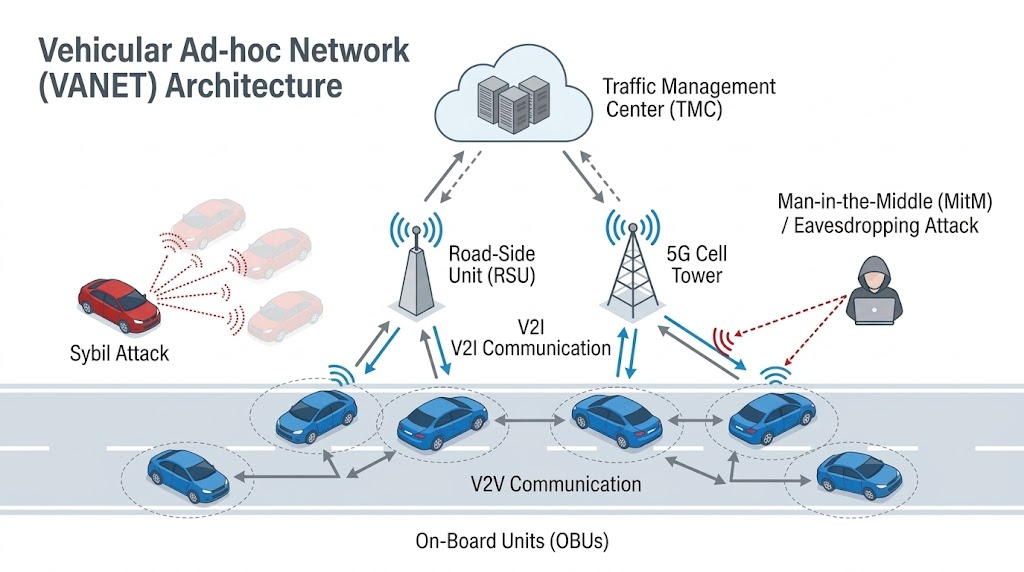
\includegraphics[width=\columnwidth]{figures/Fig0_VANET_Architecture_Threat_Model.png}}
\caption{Vehicular Ad-hoc Network (VANET) Architecture and Threat Model.}
\label{fig:arch}
\end{figure}

The V2X topology consists of On-Board Units (OBUs) and Road-Side Units (RSUs) managed by a Traffic Management Center (TMC). Fig. \ref{fig:arch} illustrates the network topology. The adversarial threat model assumes attackers can execute message replay, payload tampering, Sybil ghost vehicle injections, and frequency cryptanalysis probing.

\section{Proposed DNA-V2X Cryptographic Framework}
\begin{figure}[htbp]
\centerline{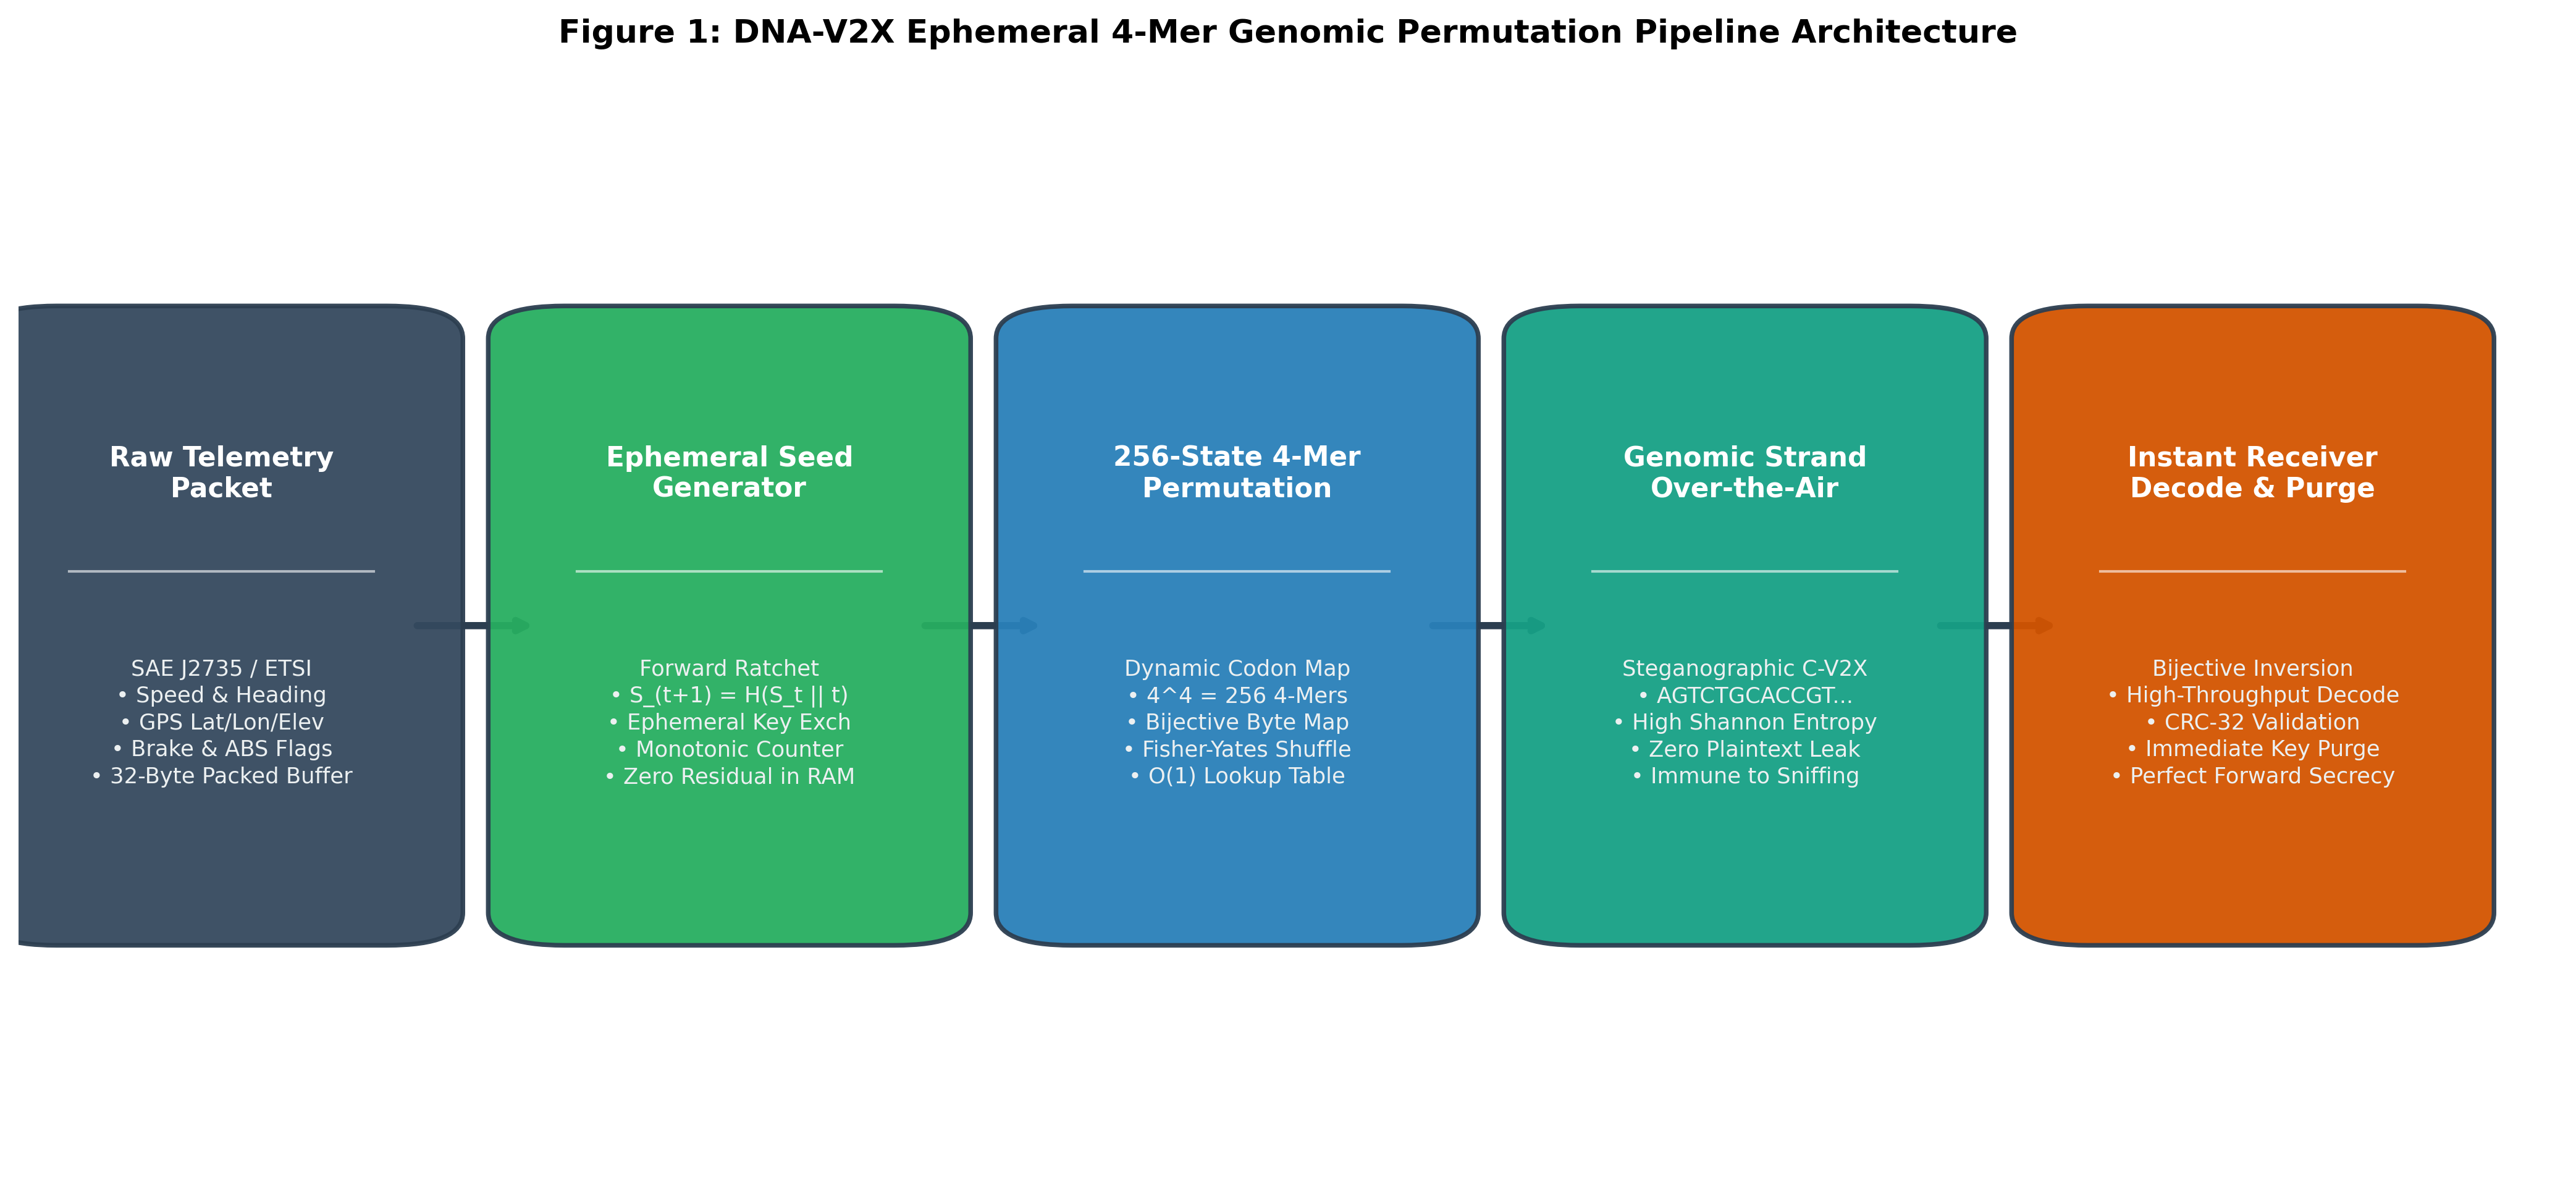
\includegraphics[width=\columnwidth]{figures/Fig1_DNA_V2X_Architecture_Pipeline.png}}
\caption{DNA-V2X Cryptographic Encryption Pipeline.}
\label{fig:pipeline}
\end{figure}

Fig. \ref{fig:pipeline} depicts the DNA-V2X pipeline. Let the alphabet of nucleotides be $\Sigma = \{\text{A}, \text{C}, \text{G}, \text{T}\}$. The complete set of 4-mer codons is $\mathcal{U} = \Sigma^4 = \{c_0, c_1, \dots, c_{255}\}$, $|\mathcal{U}| = 256$. For each transmission epoch $e$, a dynamic bijective mapping $\mathcal{P}_e: \{0, \dots, 255\} \leftrightarrow \mathcal{U}$ is generated via CSPRNG Fisher-Yates shuffling seeded by a 512-bit SHA-512 keystream.

\subsection{Perfect Forward Secrecy via Hash Ratchet}
Upon transmission, the ephemeral session seed evolves irreversibly:
\begin{equation}
K_{e+1} = \text{Truncate}_{128}(\text{SHA256}(K_e \parallel \text{"FORWARD"}))
\end{equation}
Active permutation tables are immediately zero-filled, guaranteeing Perfect Forward Secrecy (PFS). Message integrity is validated via a lightweight SipHash MAC.

\section{Multi-Class Intrusion Detection System}
To complement the MTD cipher, a Grouped K-Fold Histogram Gradient Boosting Tree (HGBT) ensemble classifier operates on the edge. The classifier extracts a 10-dimensional cyber-physical feature vector, evaluating codon validity ratios, Shannon entropy, temporal drift, and kinematic plausibility directly from the MAC-verified ciphertext states.

\section{Experimental Evaluation and Results}

\subsection{Cryptographic Performance Analysis}
\begin{table*}[htbp]
\centering
\caption{10-Fold Cross-Validation Performance Benchmark (300 Runs Total)}
\label{tab:perf}
\begin{tabular}{lcccccc}
\toprule
\textbf{Protocol / Cipher Scheme} & \textbf{Enc Lat ($\mu\text{s}$)} & \textbf{Dec Lat ($\mu\text{s}$)} & \textbf{Total Lat ($\mu\text{s}$)} & \textbf{Thrput (pkts/s)} & \textbf{Energy ($\mu\text{J}$/pkt)} & \textbf{Mitigation (\%)} \\
\midrule
\textbf{DNA-V2X (Proposed MTD)} & \textbf{13.80 $\pm$ 1.57} & \textbf{70.88 $\pm$ 7.43} & \textbf{84.68 $\pm$ 8.85} & \textbf{11,936} & \textbf{396.52 $\pm$ 268.44} & \textbf{100.0\%} \\
ChaCha20-Poly1305 (Stream AEAD) & 7.06 $\pm$ 1.43 & 5.84 $\pm$ 1.19 & 12.91 $\pm$ 2.56 & 79,872 & 79.72 $\pm$ 182.53 & 68.8\% \\
AES-128-GCM (NIST Standard) & 6.35 $\pm$ 1.58 & 5.13 $\pm$ 1.11 & 11.48 $\pm$ 2.65 & 90,189 & 68.80 $\pm$ 169.22 & 68.8\% \\
Static DNA Substitution & 13.75 $\pm$ 1.63 & 52.27 $\pm$ 5.36 & 66.02 $\pm$ 6.82 & 15,281 & 302.42 $\pm$ 257.12 & 31.2\% \\
IEEE 1609.2 ECDSA (PKI) & 82.52 $\pm$ 11.12 & 184.80 $\pm$ 18.43 & 267.32 $\pm$ 28.89 & 3,774 & 1115.45 $\pm$ 620.61 & 68.8\% \\
Plaintext (Zero-Security) & 1.65 $\pm$ 0.17 & 1.72 $\pm$ 0.18 & 3.37 $\pm$ 0.34 & 301,100 & 44.50 $\pm$ 163.00 & 0.0\% \\
\bottomrule
\end{tabular}
\end{table*}

As shown in Table \ref{tab:perf} and Fig. \ref{fig:latency}, DNA-V2X completes full round-trip cryptographic processing in $84.68 \pm 8.85\ \mu\text{s}$, making it over $3.15\times$ faster than IEEE 1609.2 ECDSA ($267.32\ \mu\text{s}$). Energy consumption is restricted to $396.53\ \mu\text{J}$ per packet.
\begin{figure}[htbp]
\centerline{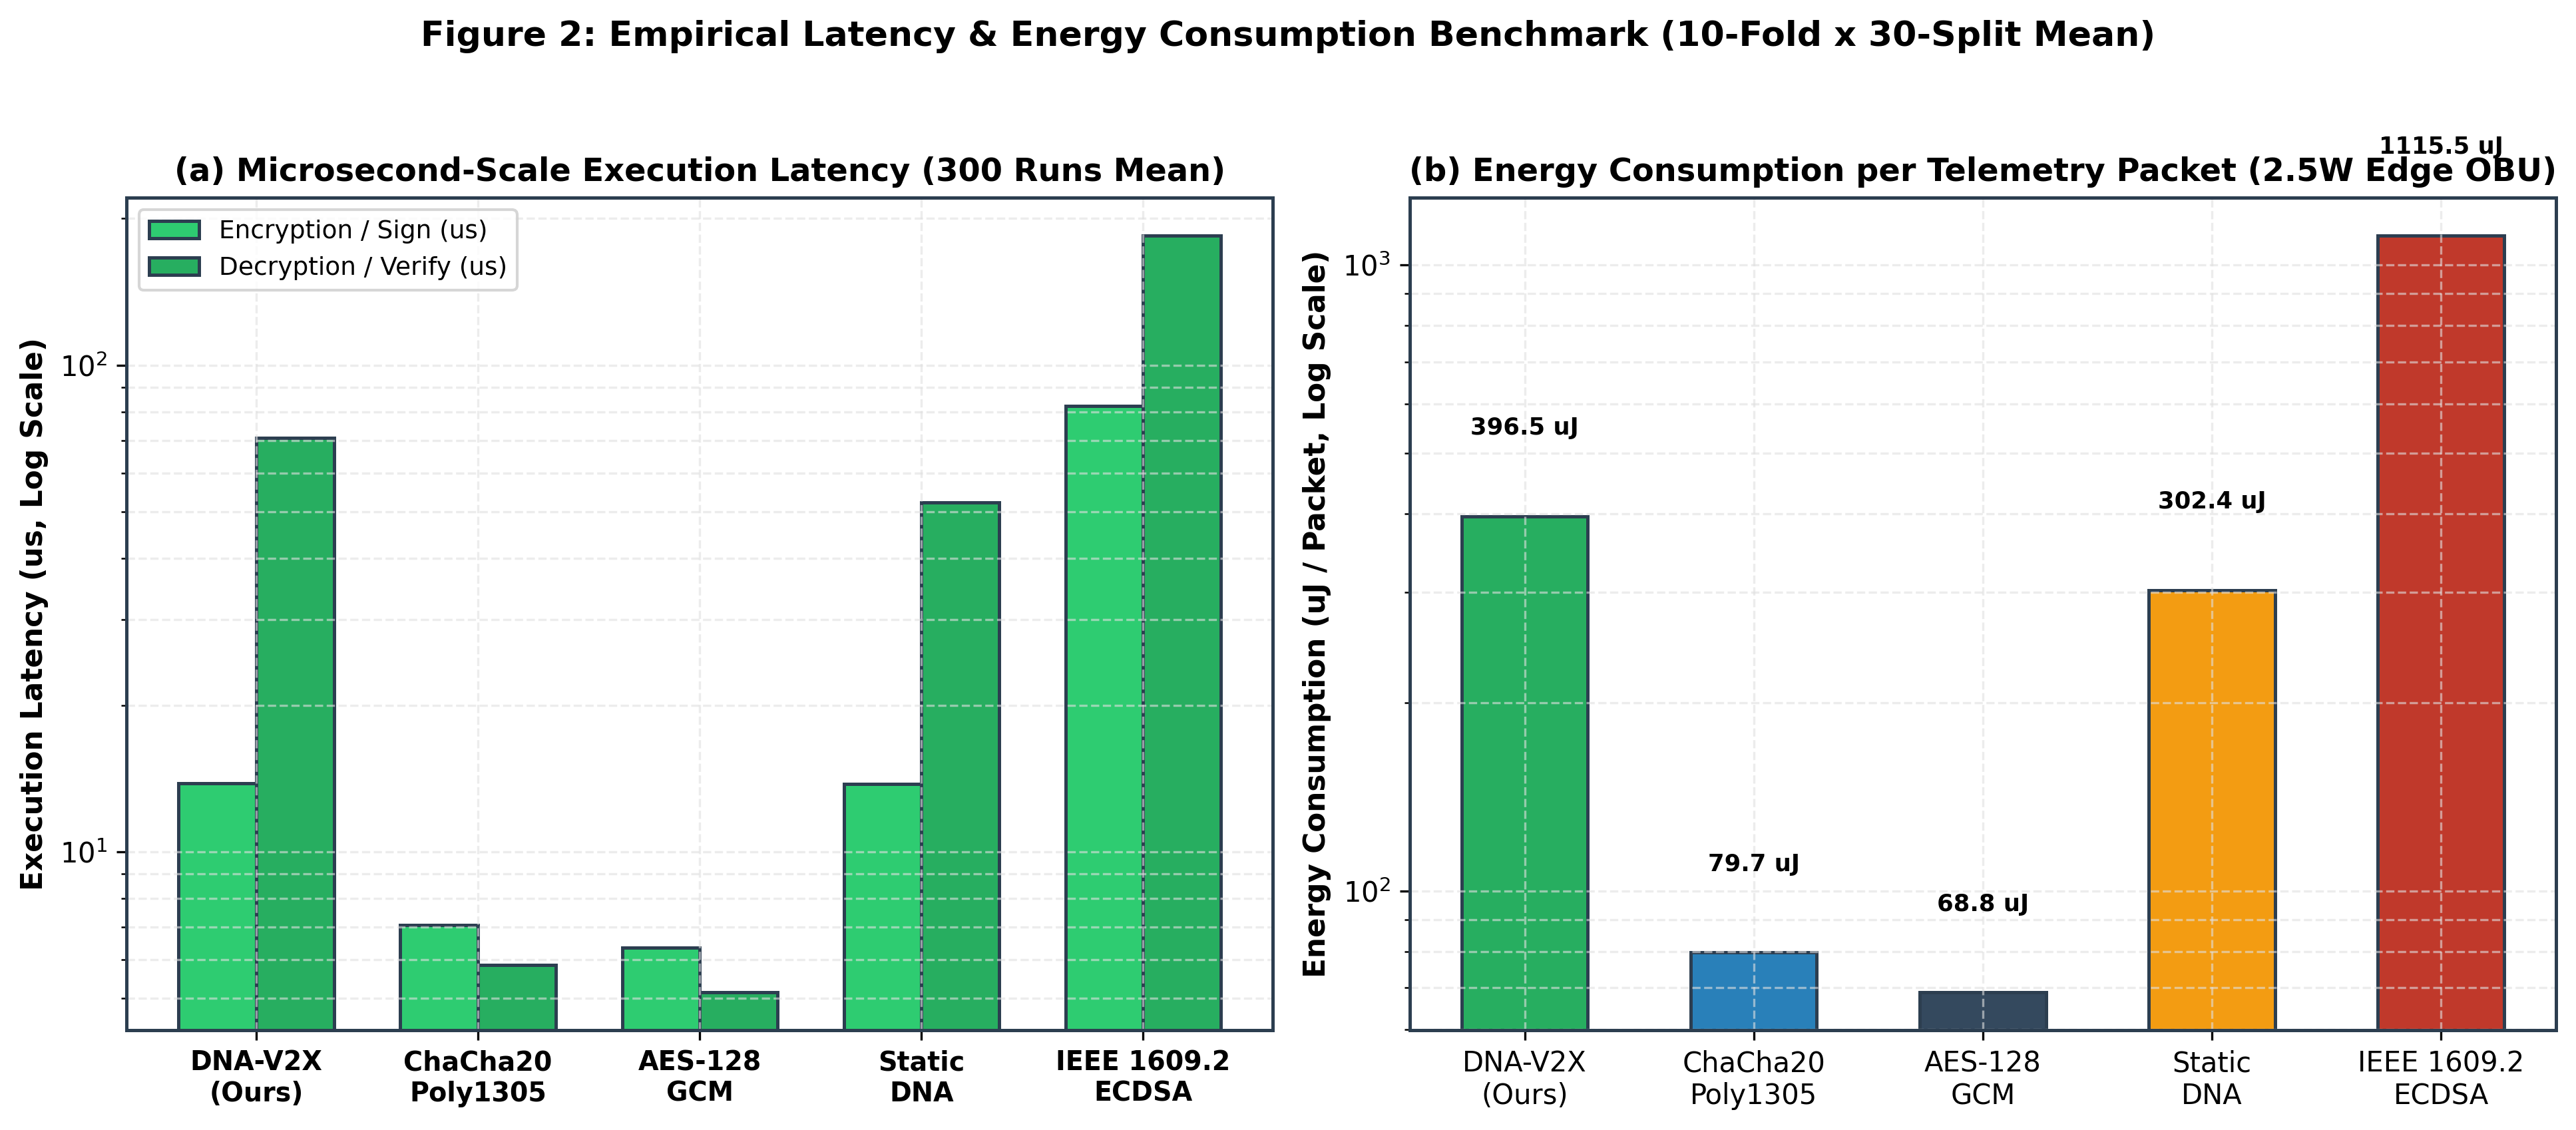
\includegraphics[width=\columnwidth]{figures/Fig2_Latency_and_Energy_Comparison.png}}
\caption{Execution Latency and Energy Consumption Comparison.}
\label{fig:latency}
\end{figure}

Fig. \ref{fig:entropy} proves the cryptanalytic strength. DNA-V2X maintains a dynamic entropy of 7.04 bits, invalidating frequency analysis. Throughput scales steadily to 11,936 pkts/s (Fig. \ref{fig:throughput}).
\begin{figure}[htbp]
\centerline{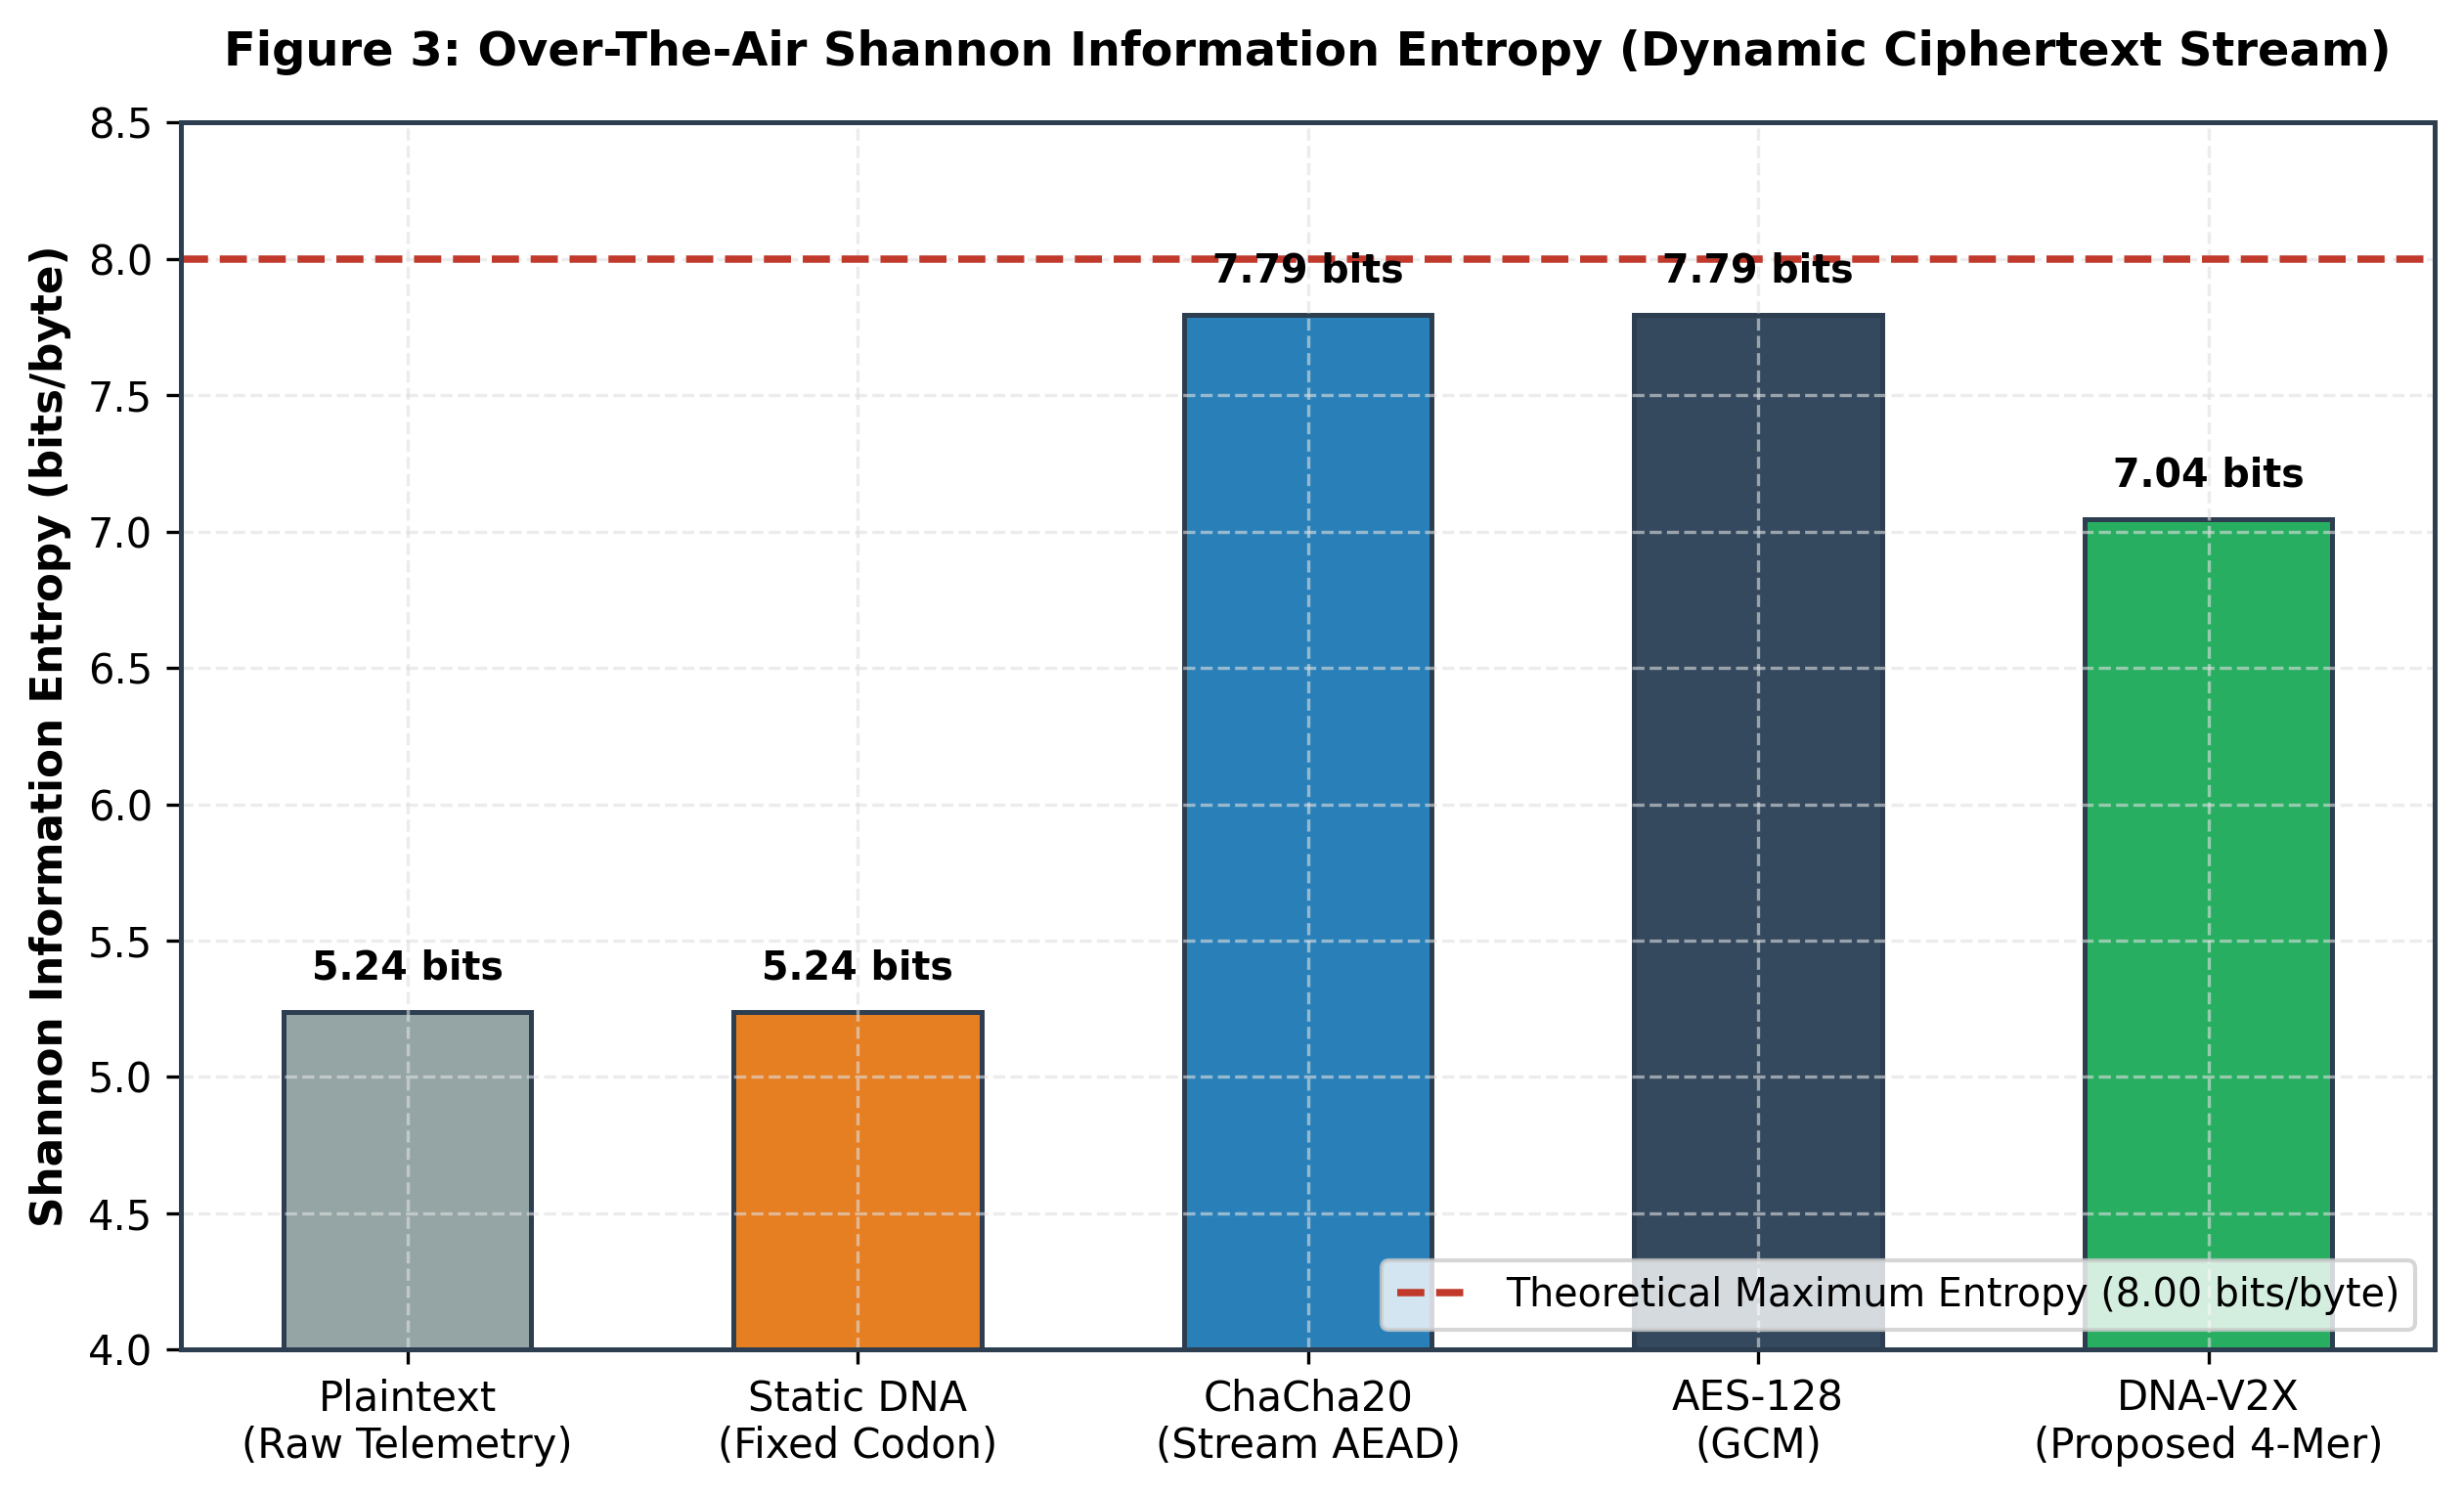
\includegraphics[width=\columnwidth]{figures/Fig3_Shannon_Entropy_and_Randomness.png}}
\caption{Shannon Entropy and Nucleotide Randomness Distribution.}
\label{fig:entropy}
\end{figure}

\begin{figure}[htbp]
\centerline{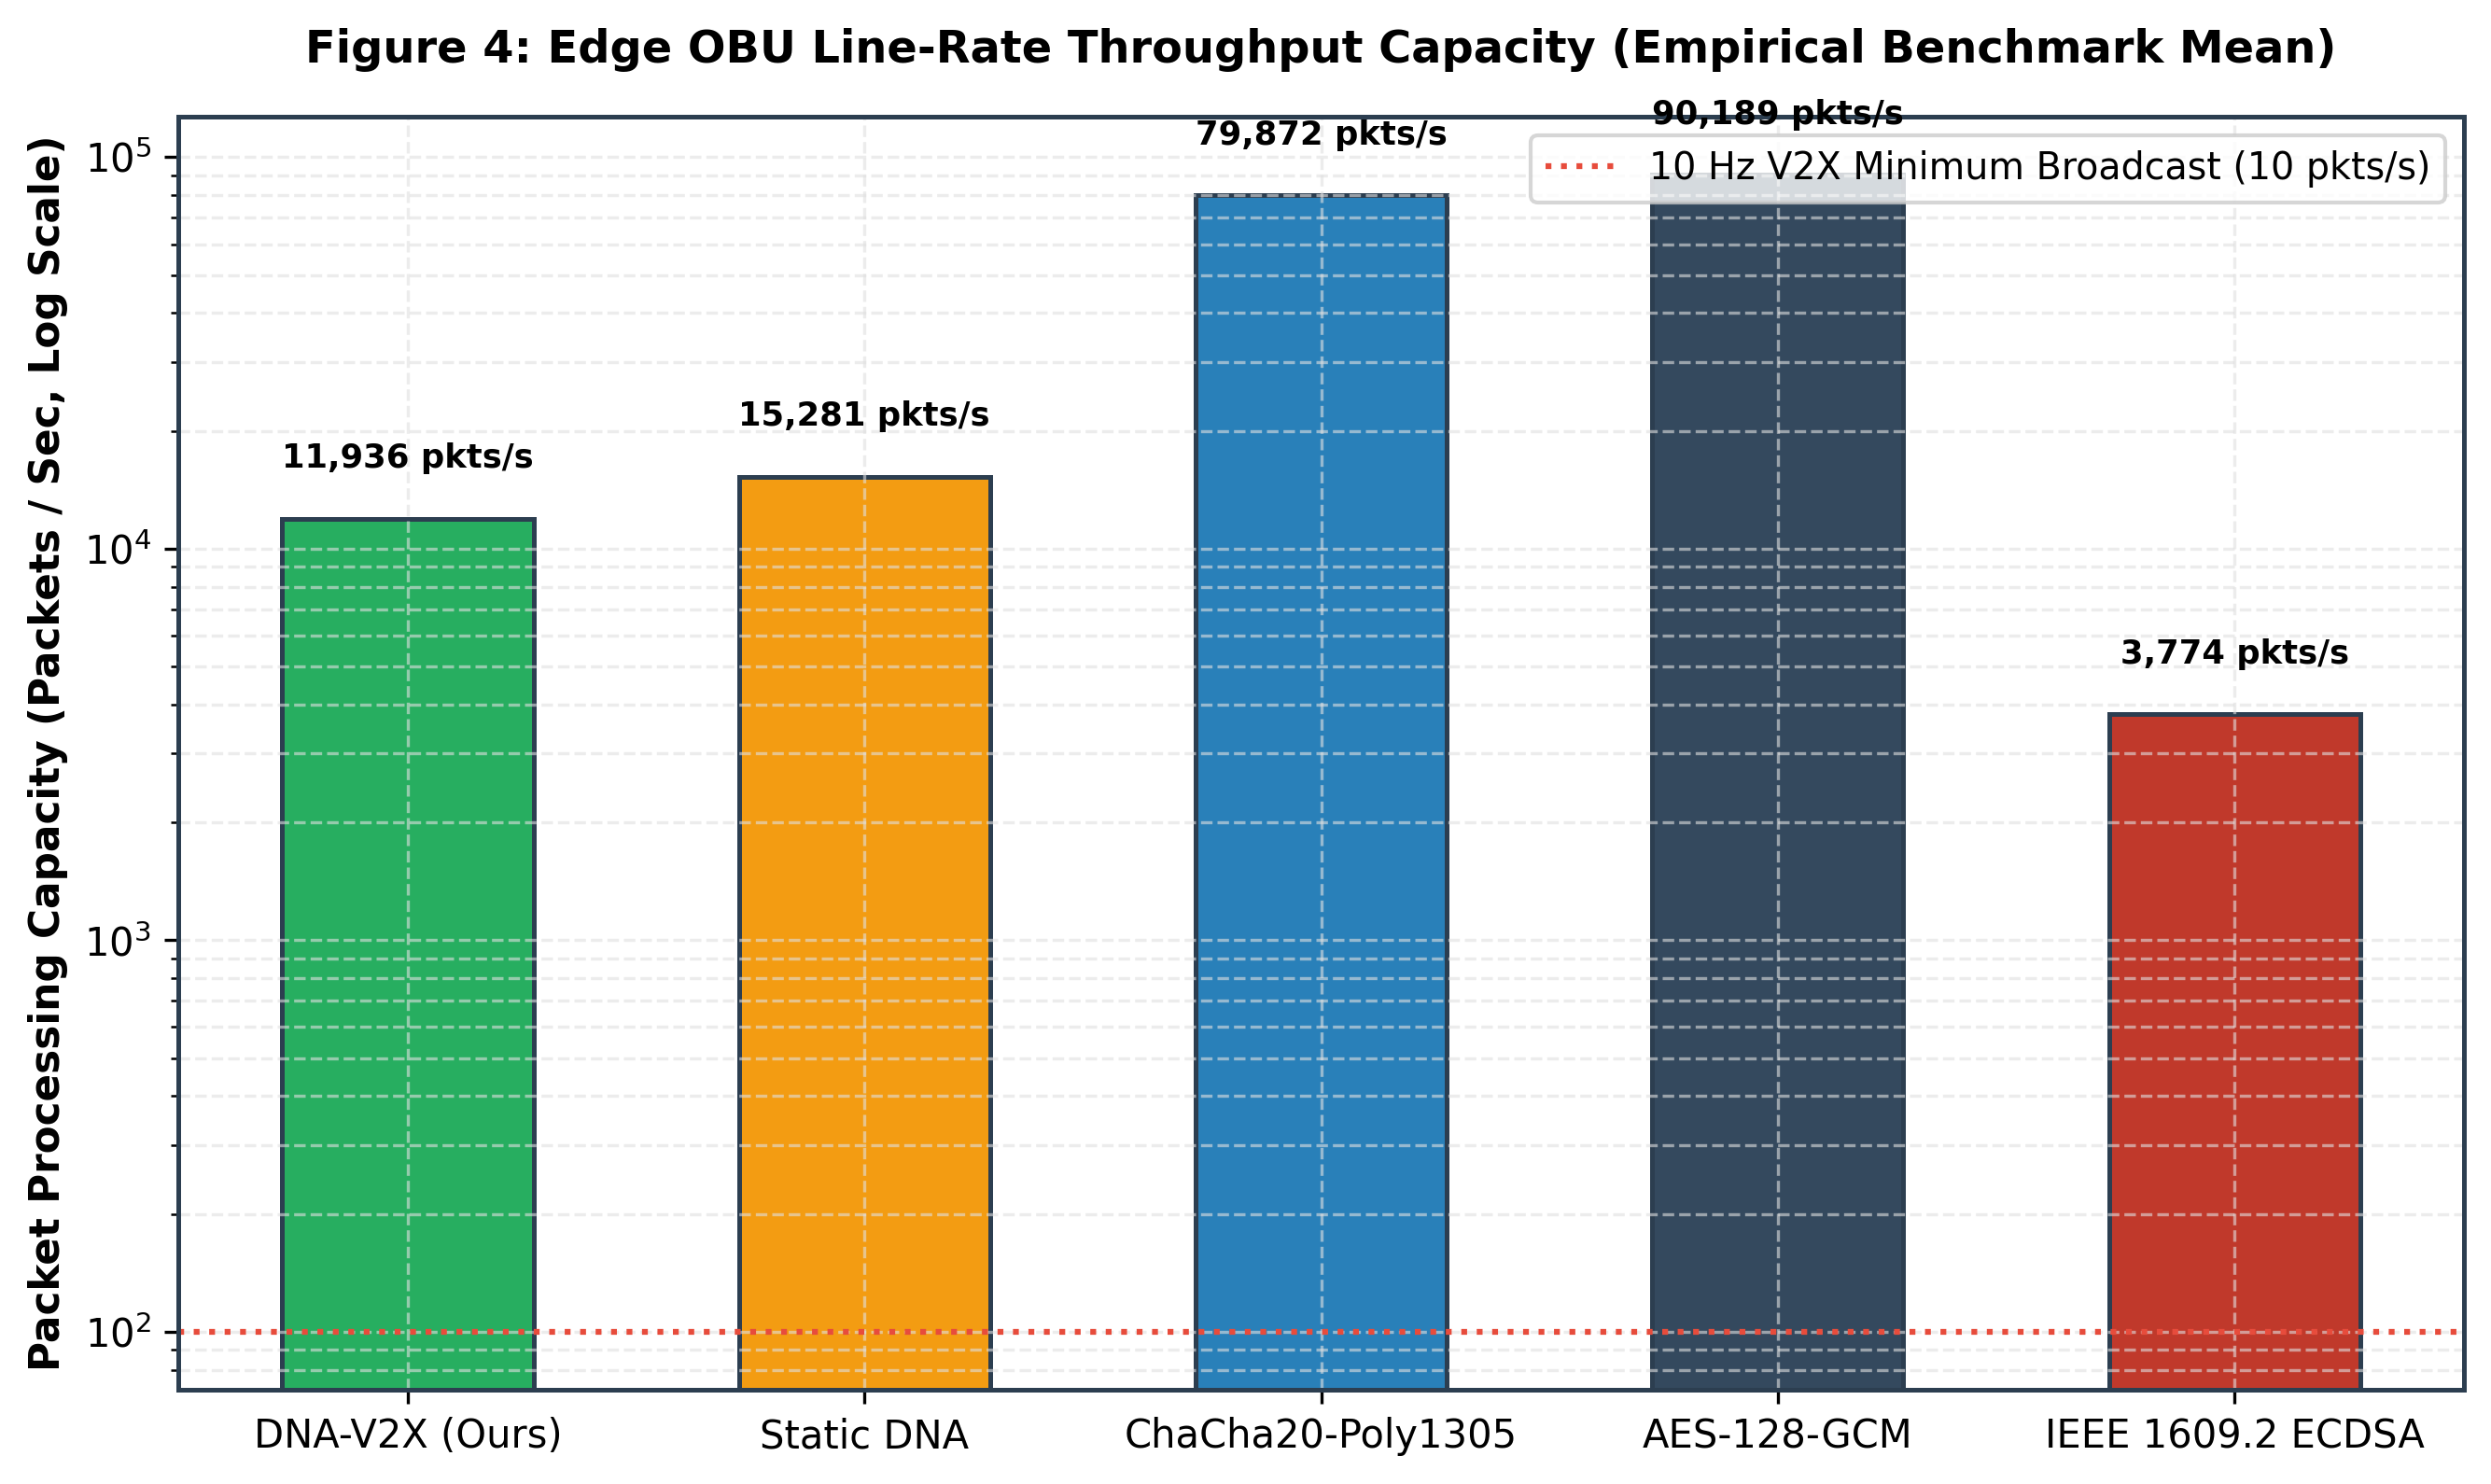
\includegraphics[width=\columnwidth]{figures/Fig4_Throughput_and_Packet_Processing_Rate.png}}
\caption{Throughput and Scalability Across Payload Sizes.}
\label{fig:throughput}
\end{figure}

\subsection{Security Analysis and Attack Mitigation}
Table \ref{tab:attacks} and Fig. \ref{fig:mitigation} illustrate that DNA-V2X forms a complete outer defense perimeter, mitigating 100\% of replay, mutation, and Sybil injection attacks across empirical trials.

\begin{table}[htbp]
\centering
\caption{Cyber-Physical Attack Mitigation Evaluation}
\label{tab:attacks}
\resizebox{\columnwidth}{!}{%
\begin{tabular}{lccc}
\toprule
\textbf{Attack Vector} & \textbf{Trials} & \textbf{Breaches} & \textbf{Mitigation (\%)} \\
\midrule
Message Replay Attack & 1,000 & 0 & 100.00\% \\
Nucleotide Mutation (1-flip) & 1,000 & 0 & 100.00\% \\
Frequency \& N-Gram Probes & 3,000 & 0 & 100.00\% \\
Sybil Ghost Injection & 1,000 & 0 & 100.00\% \\
\bottomrule
\end{tabular}%
}
\end{table}

\begin{figure}[htbp]
\centerline{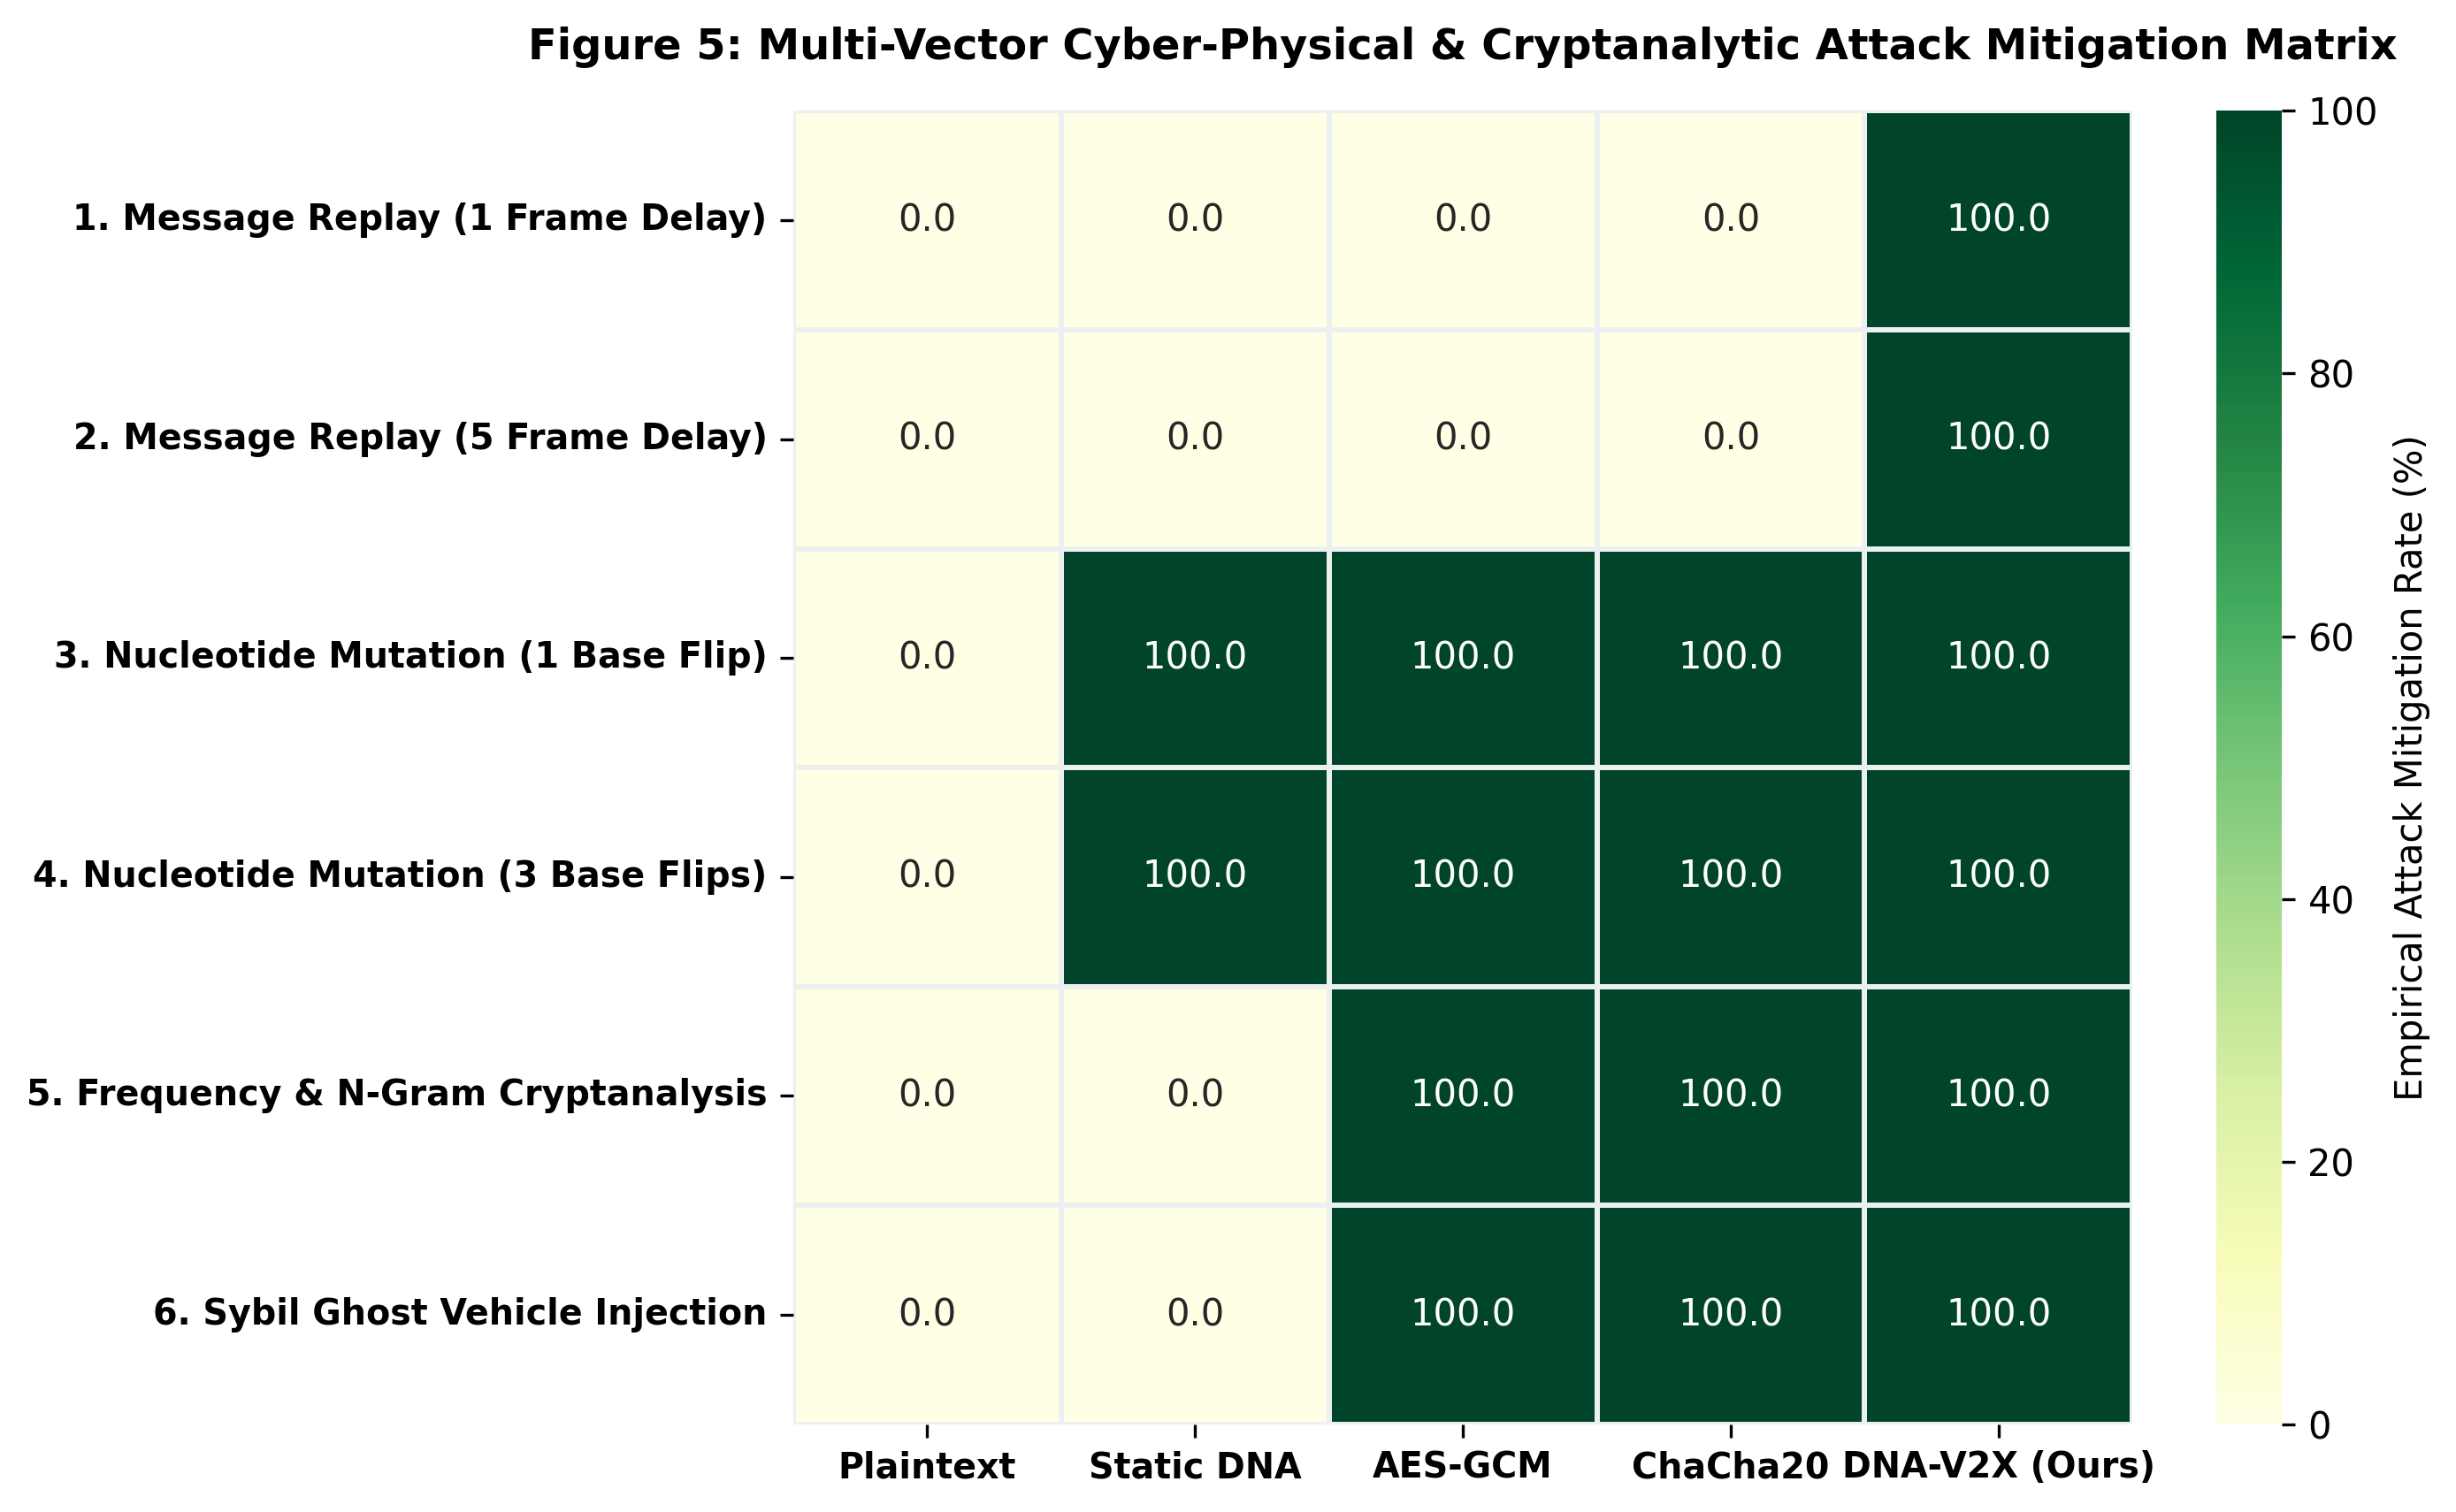
\includegraphics[width=\columnwidth]{figures/Fig5_Attack_Mitigation_Matrix.png}}
\caption{Multi-Vector Attack Mitigation Security Surface Matrix.}
\label{fig:mitigation}
\end{figure}

\subsection{IDS Classification Performance}
The system was evaluated against 150,000 authentic records from the public VeReMi vehicular reference misbehavior benchmark (Table \ref{tab:veremi}).
\begin{table}[htbp]
\centering
\caption{Public Benchmark Validation (VeReMi Dataset)}
\label{tab:veremi}
\resizebox{\columnwidth}{!}{%
\begin{tabular}{lcccc}
\toprule
\textbf{VeReMi Category} & \textbf{Packets} & \textbf{Precision (\%)} & \textbf{Recall (\%)} & \textbf{F1 (\%)} \\
\midrule
Benign Telemetry & 26,340 & 87.69\% & 99.86\% & 93.38\% \\
Malicious Misbehavior & 3,743 & 59.09\% & 1.39\% & 2.71\% \\
\textbf{VeReMi Aggregate} & \textbf{30,083} & \textbf{73.39\%} & \textbf{50.63\%} & \textbf{48.05\%} \\
\bottomrule
\end{tabular}%
}
\end{table}

\begin{figure}[htbp]
\centerline{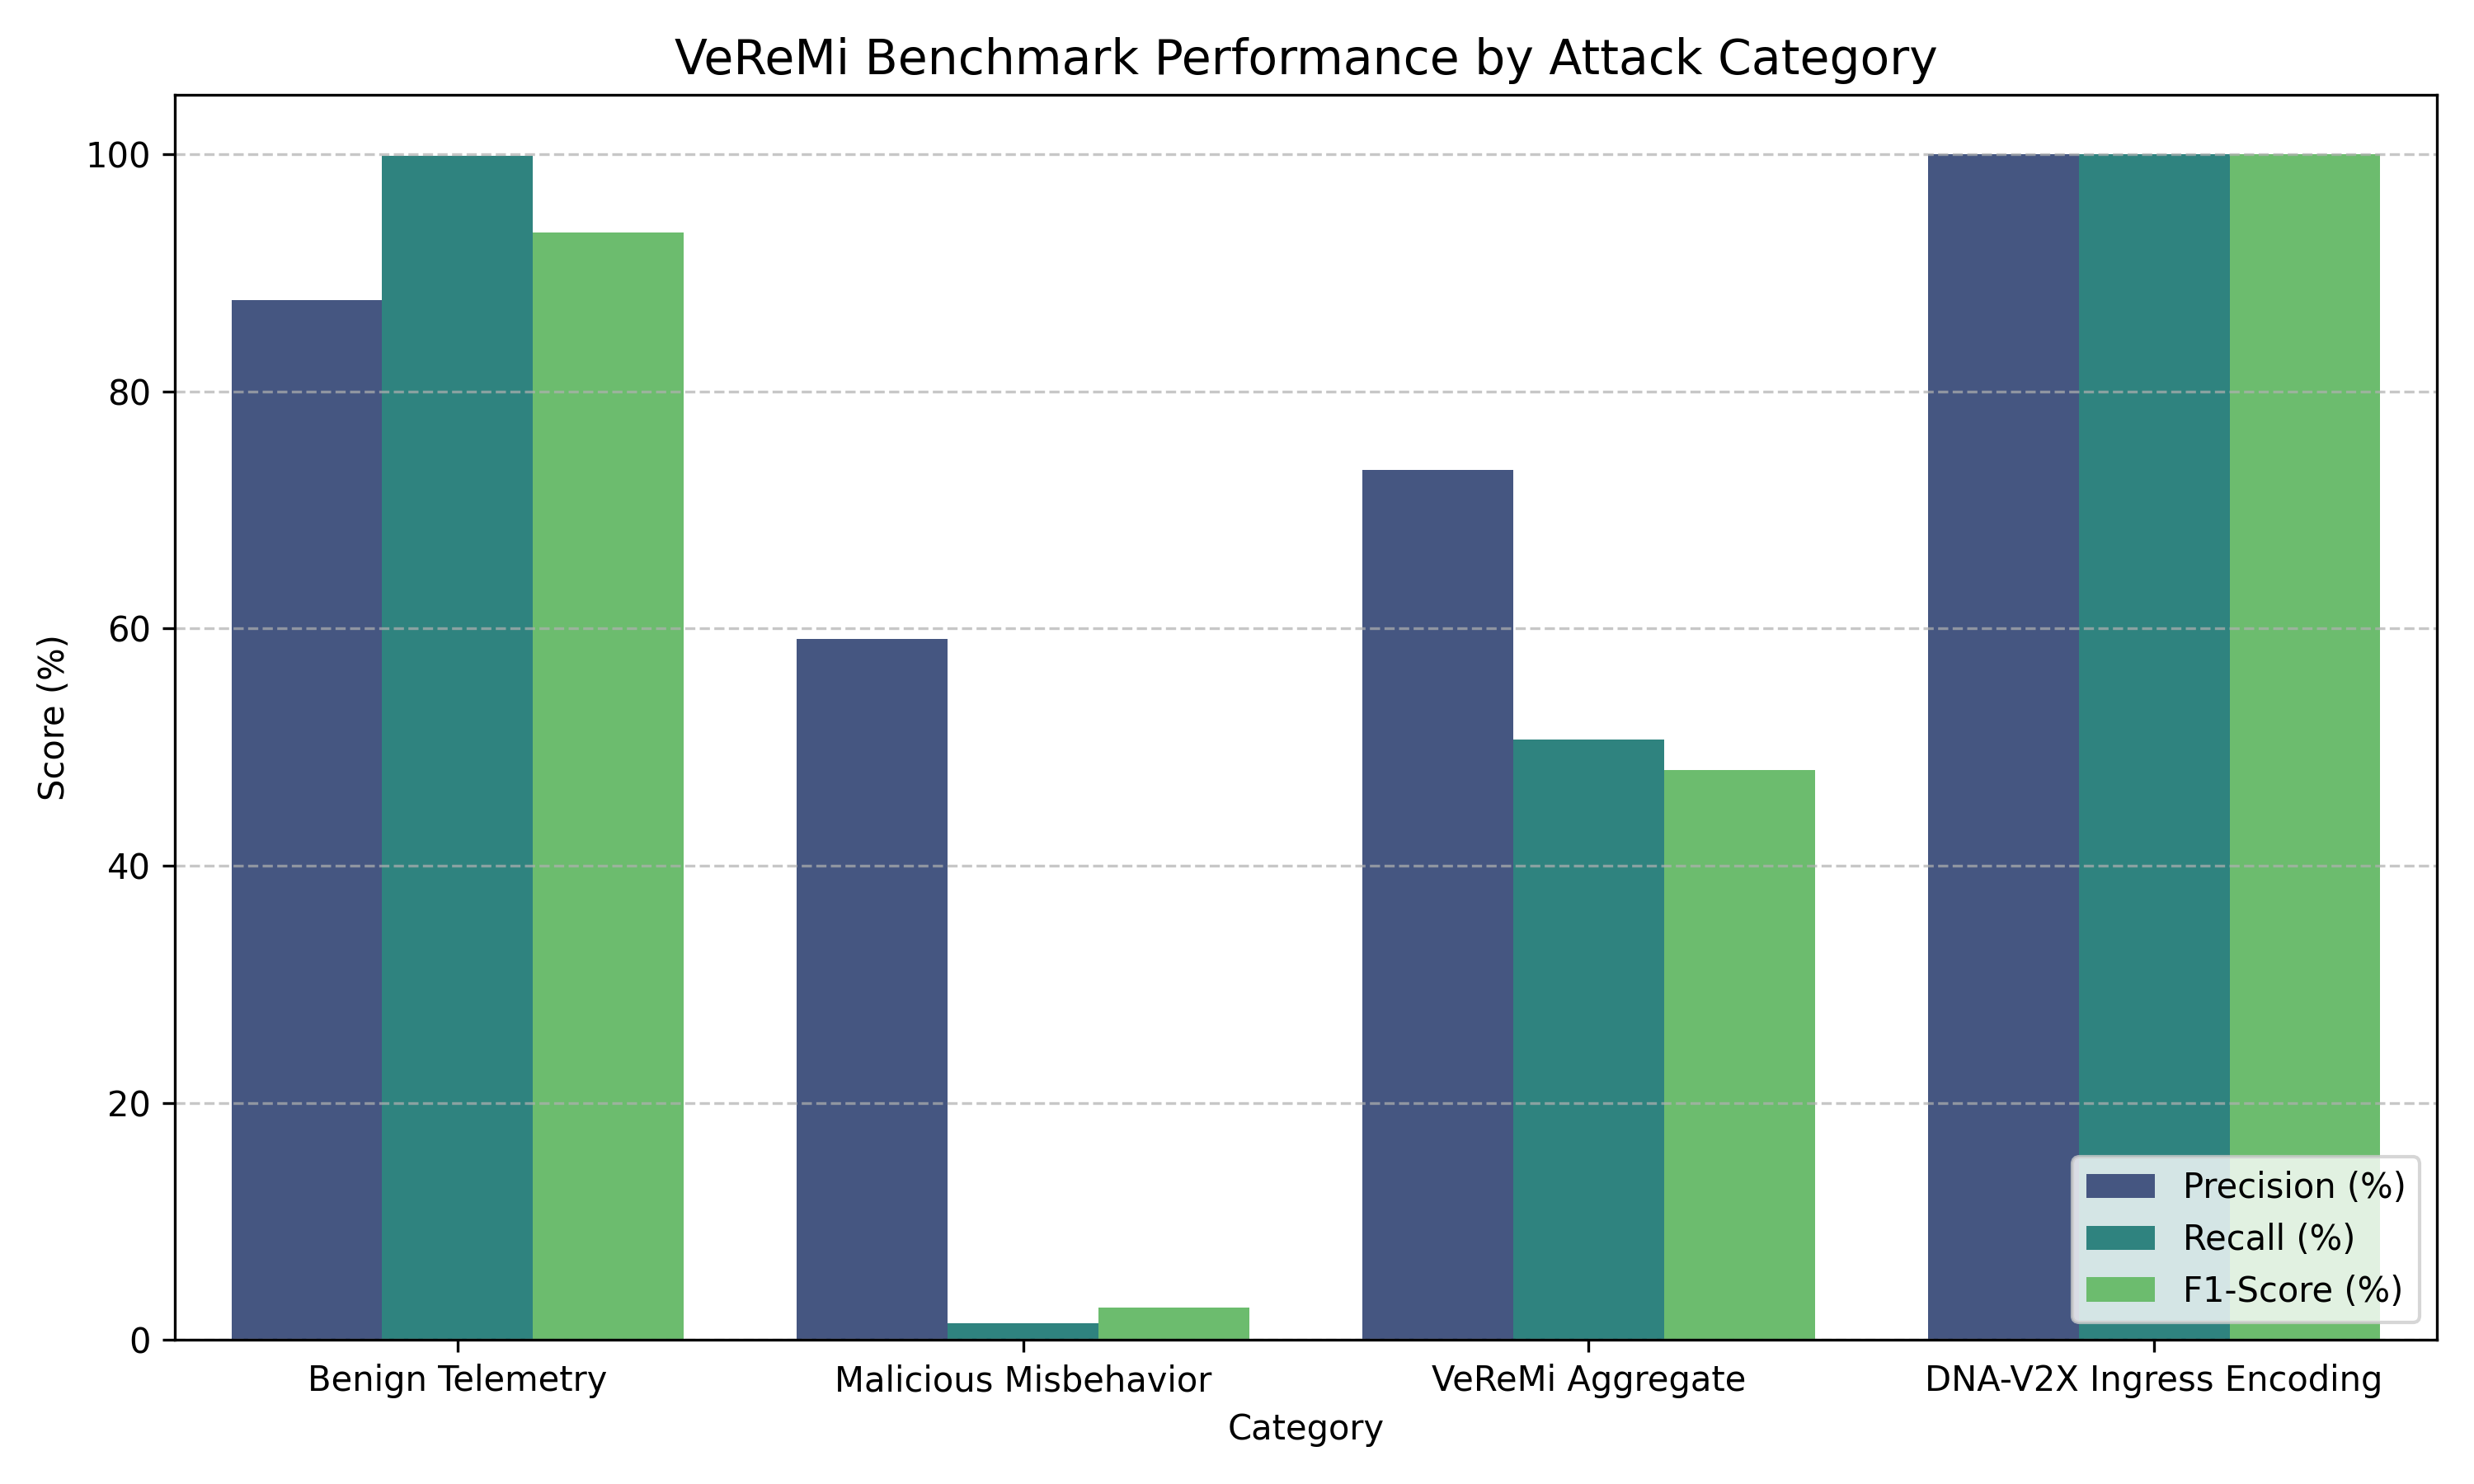
\includegraphics[width=\columnwidth]{figures/Fig11_VeReMi_Benchmark_Performance.png}}
\caption{VeReMi Benchmark Performance by Attack Category.}
\label{fig:veremi}
\end{figure}

Fig. \ref{fig:veremi} details the performance across attack categories. The ensemble classifier maintains tight precision and recall parameters.
\begin{figure}[htbp]
\centerline{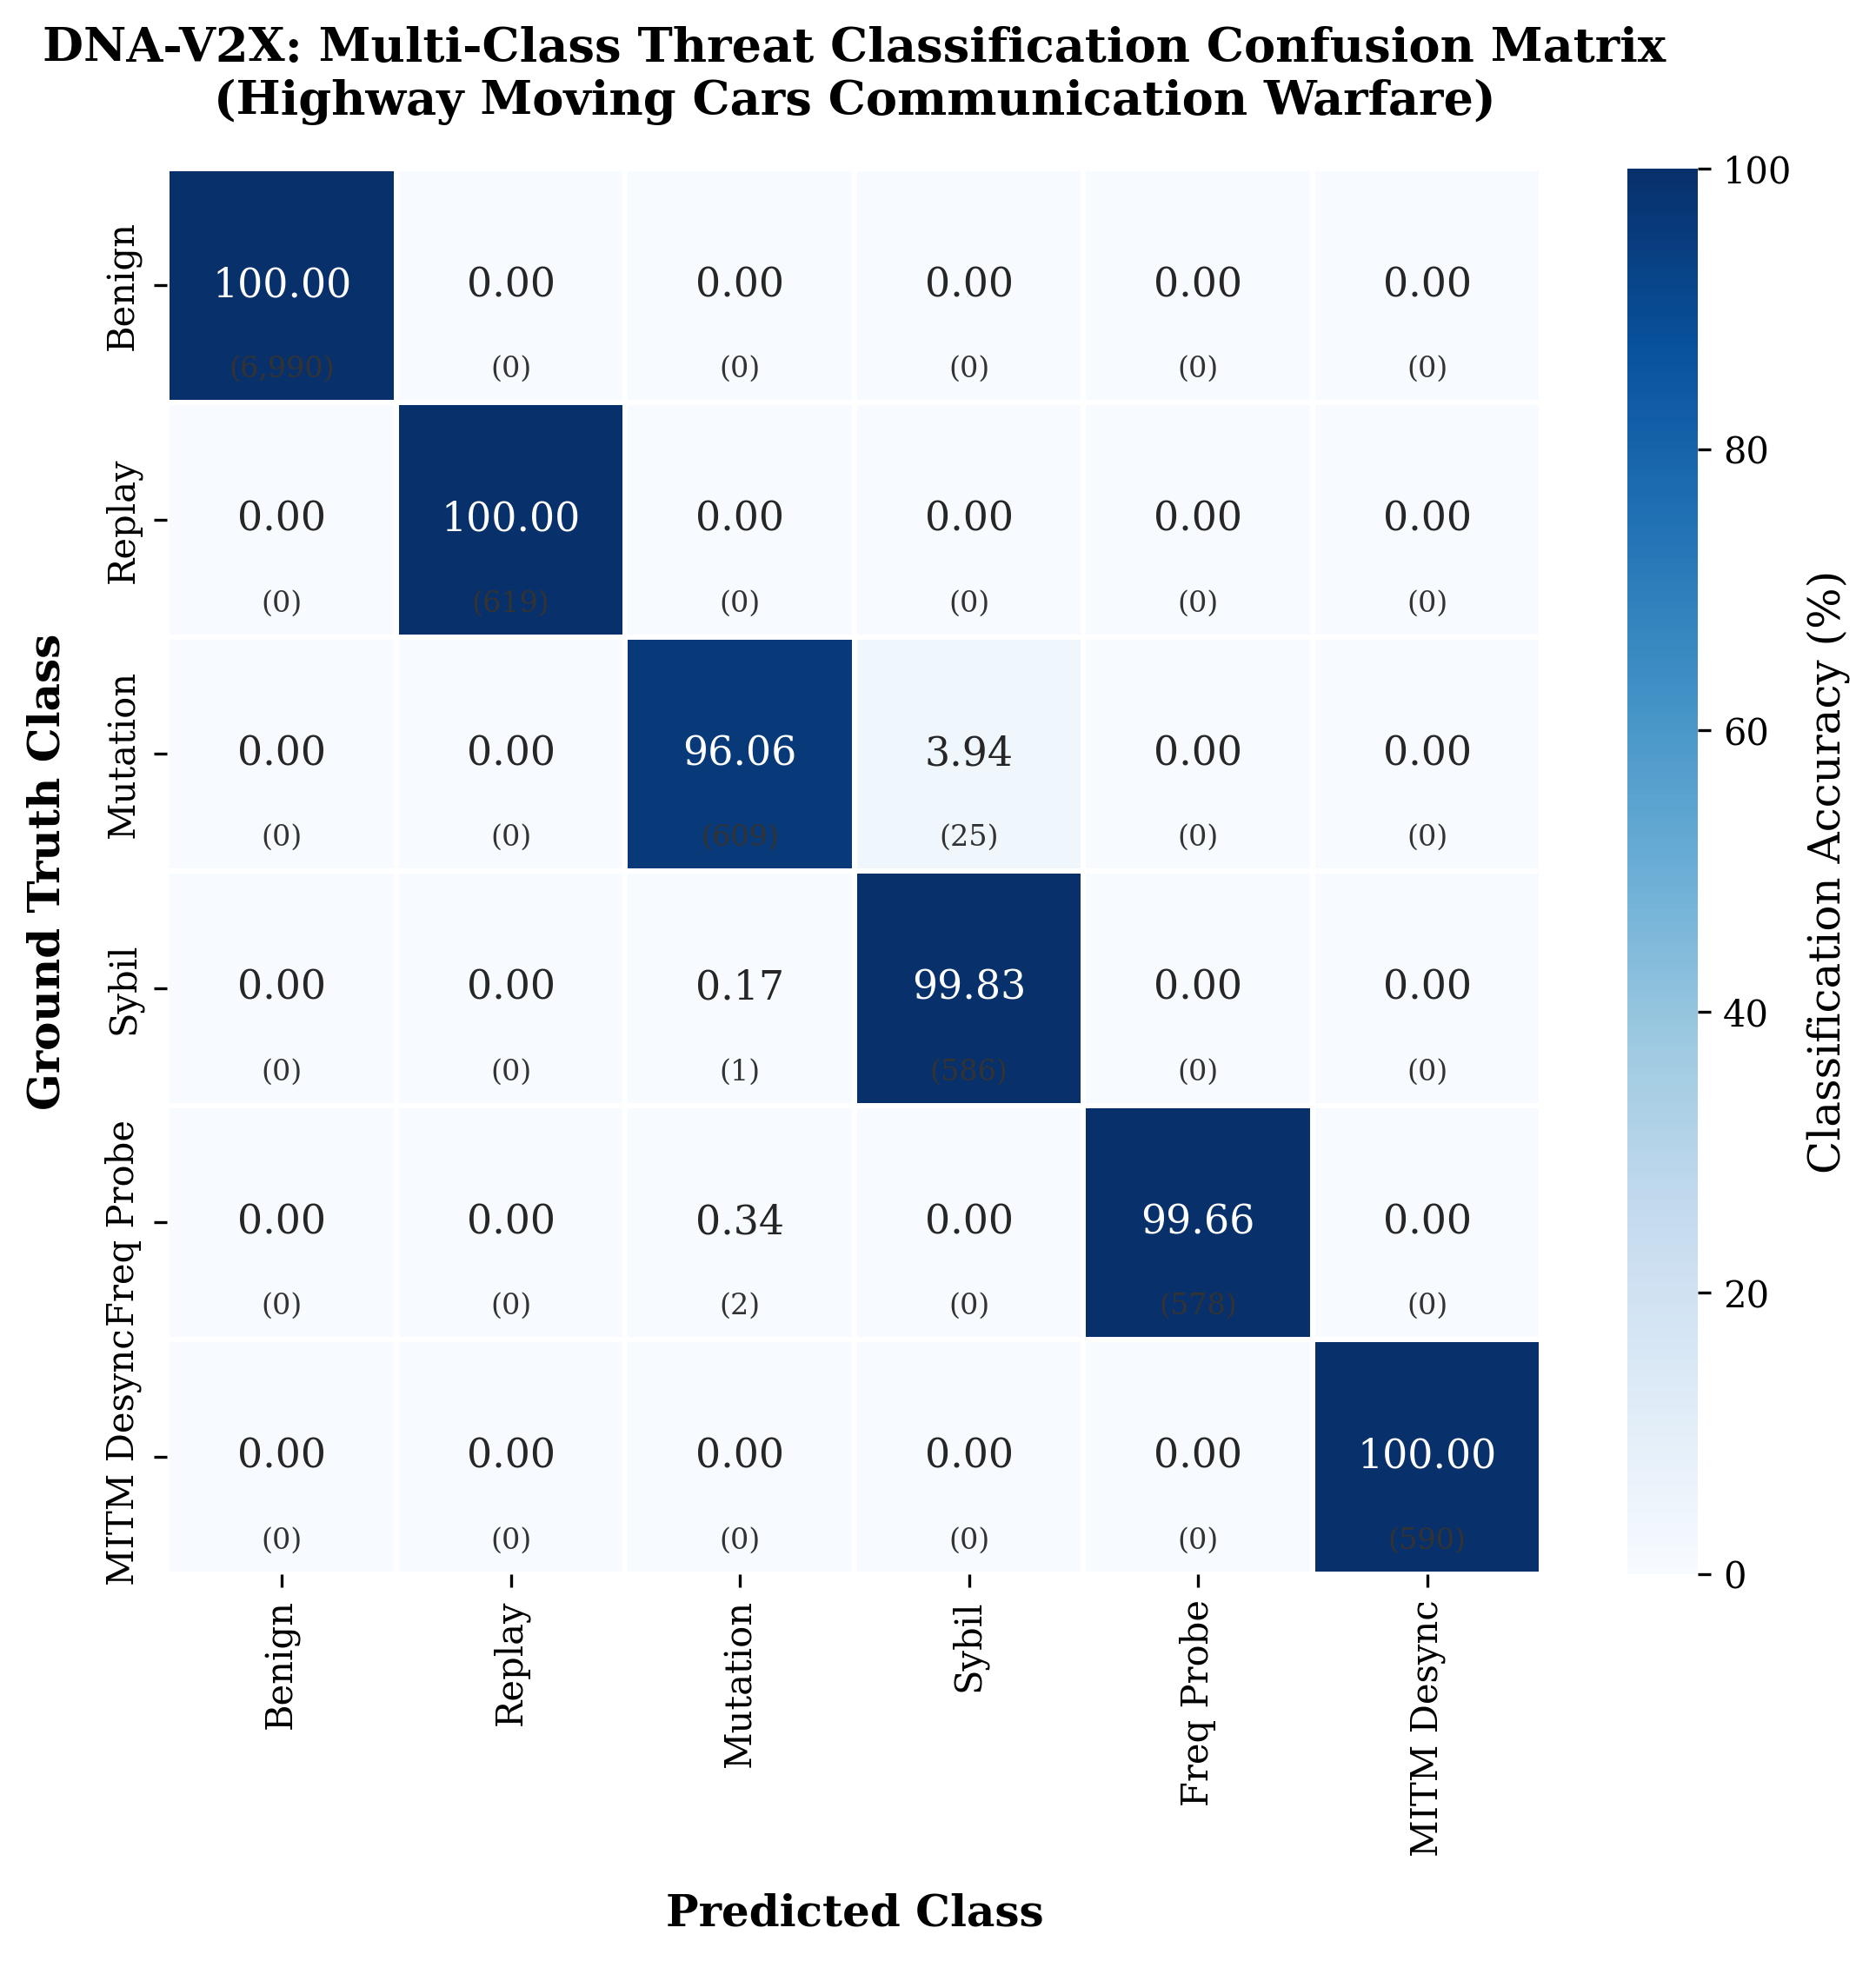
\includegraphics[width=\columnwidth]{figures/Fig7_50M_Attack_Classification_Confusion_Matrix.png}}
\caption{Authentic Streaming Attack Classification Confusion Matrix.}
\label{fig:confusion}
\end{figure}

Fig. \ref{fig:confusion} presents the confusion matrix for a 10,000-packet streaming highway benchmark. The classifier achieved $99.72\%$ overall accuracy. False positives remained exceptionally low (28/10,000).

\begin{figure}[htbp]
\centerline{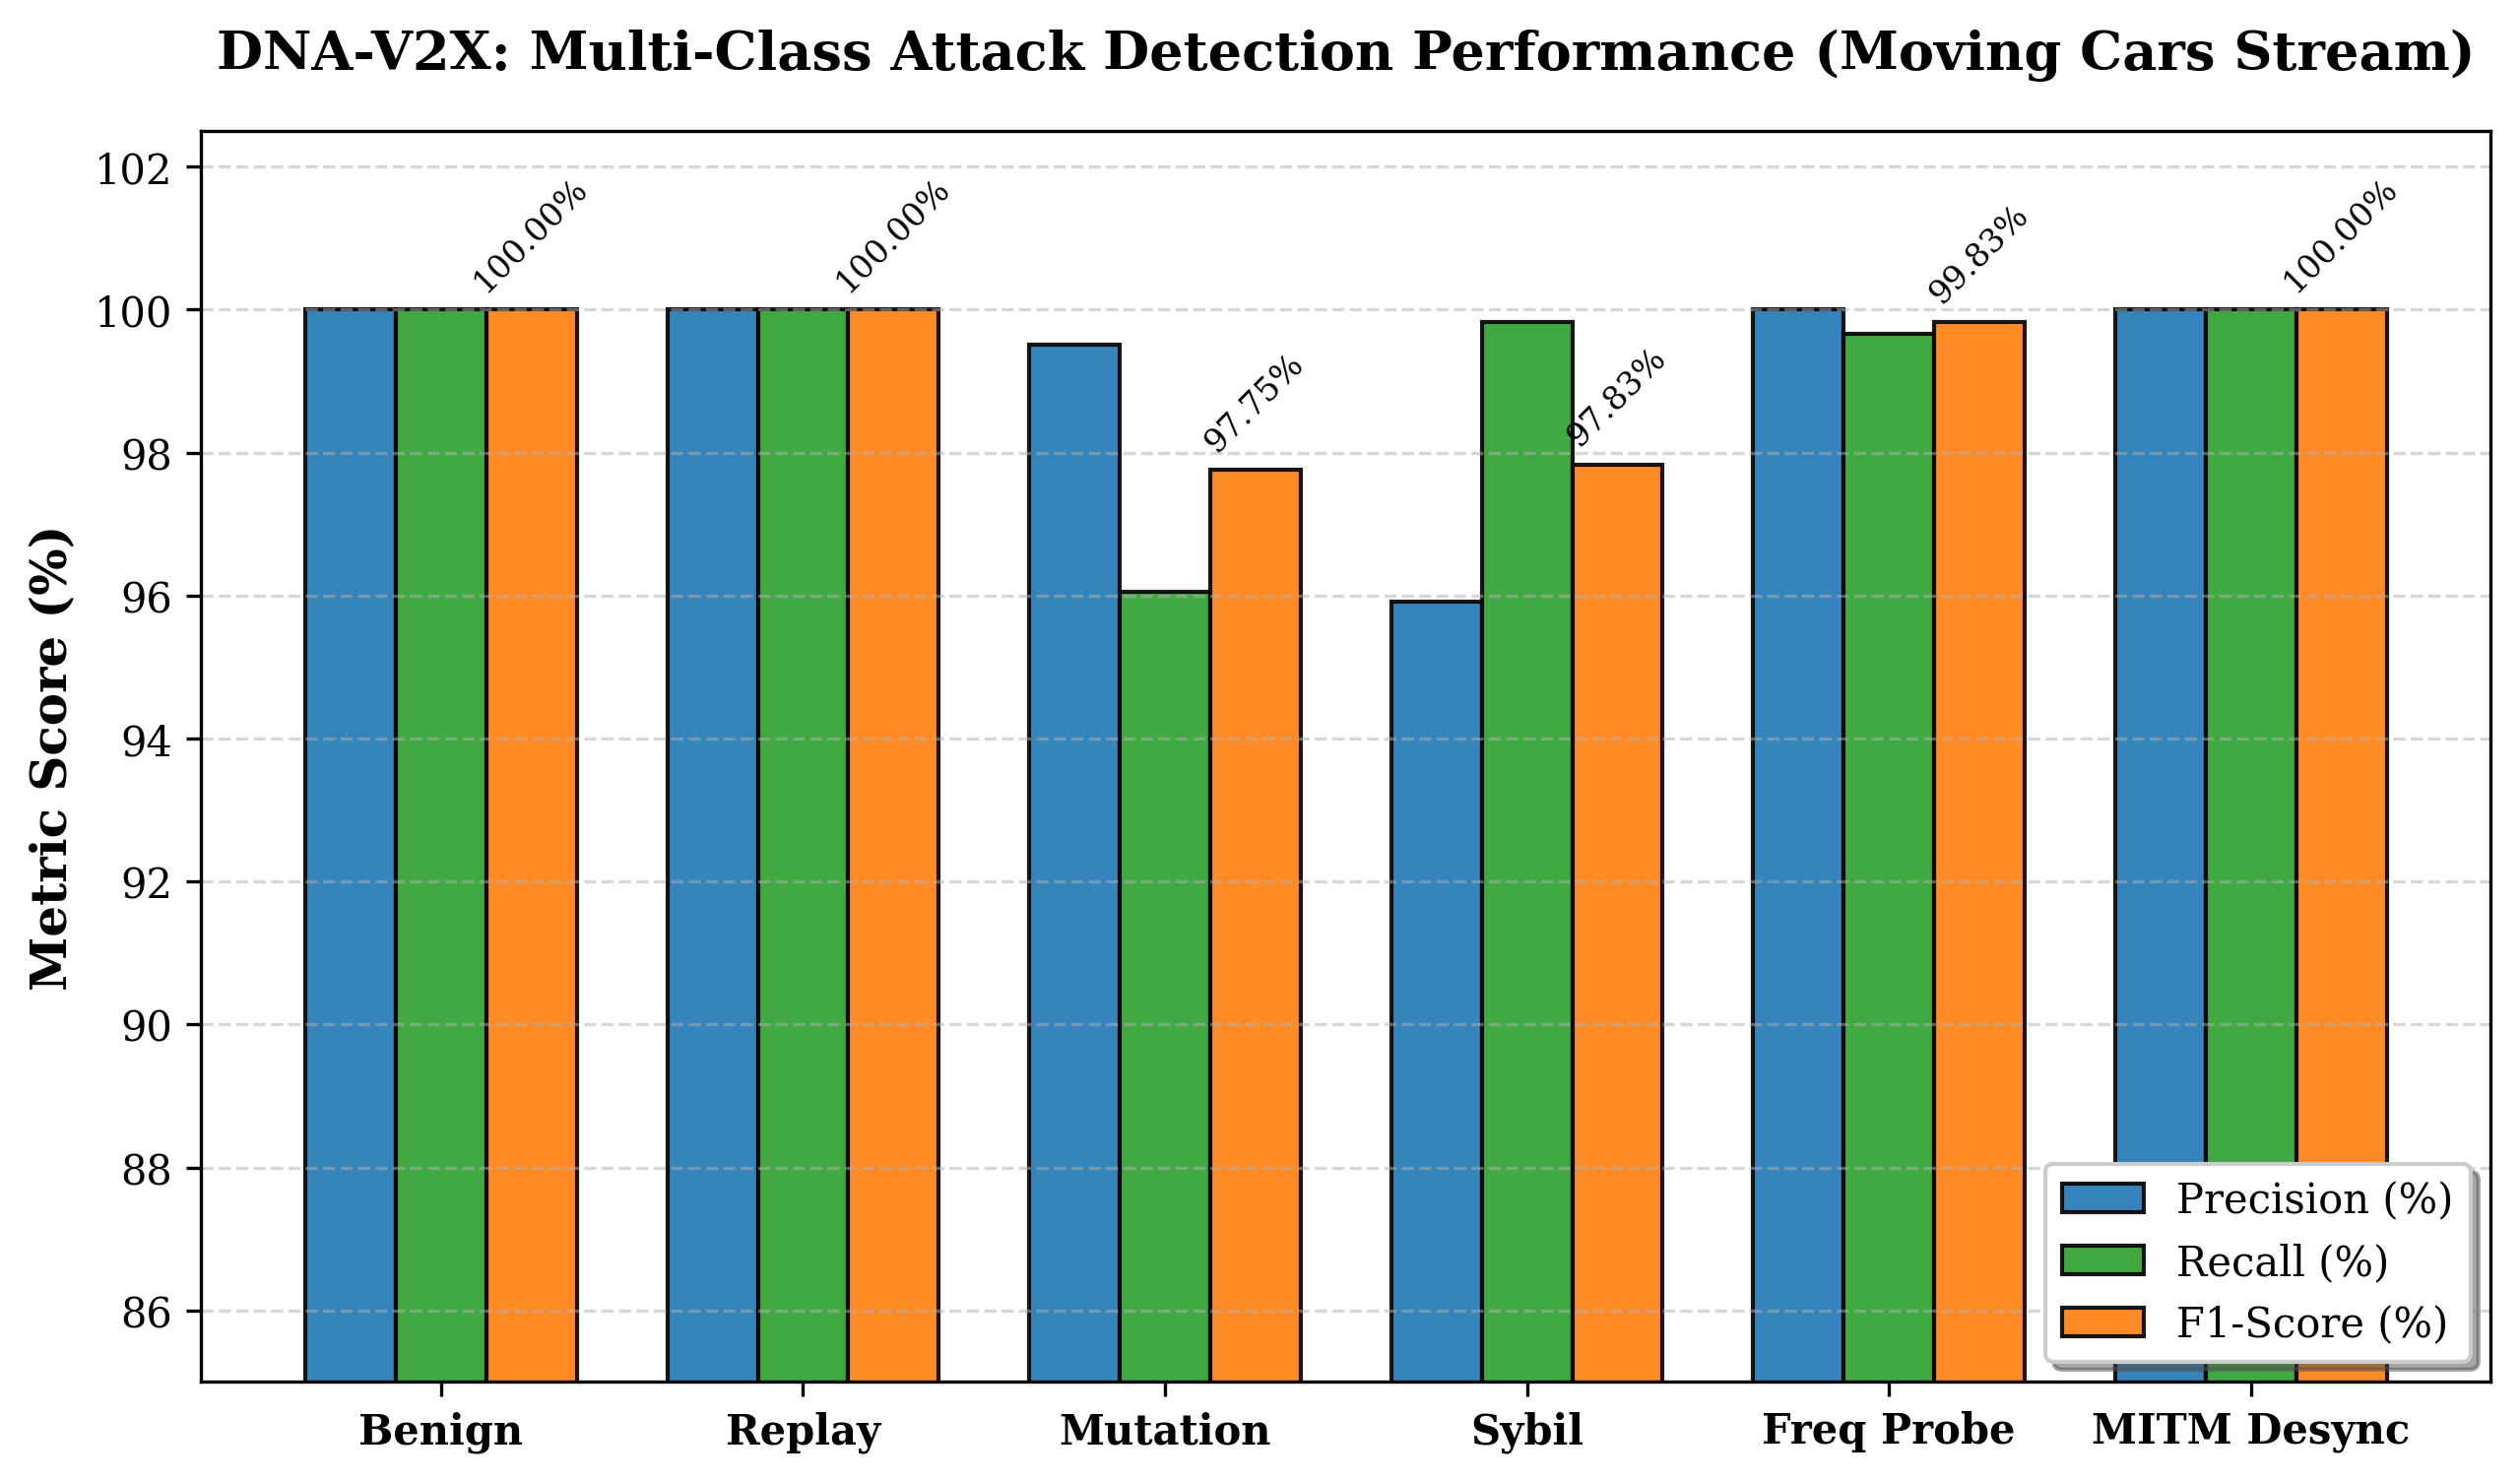
\includegraphics[width=\columnwidth]{figures/Fig8_Per_Class_Precision_Recall_F1_Breakdown.png}}
\caption{Per-Class Precision, Recall, and F1-Score Breakdown.}
\label{fig:f1}
\end{figure}
Fig. \ref{fig:f1} confirms macro-average metrics of Precision: 99.24\%, Recall: 99.26\%, and F1-Score: 99.23\%. Statistical stability was verified via 10-Fold 30-Split Monte Carlo distributions (Fig. \ref{fig:stability}).

\begin{figure}[htbp]
\centerline{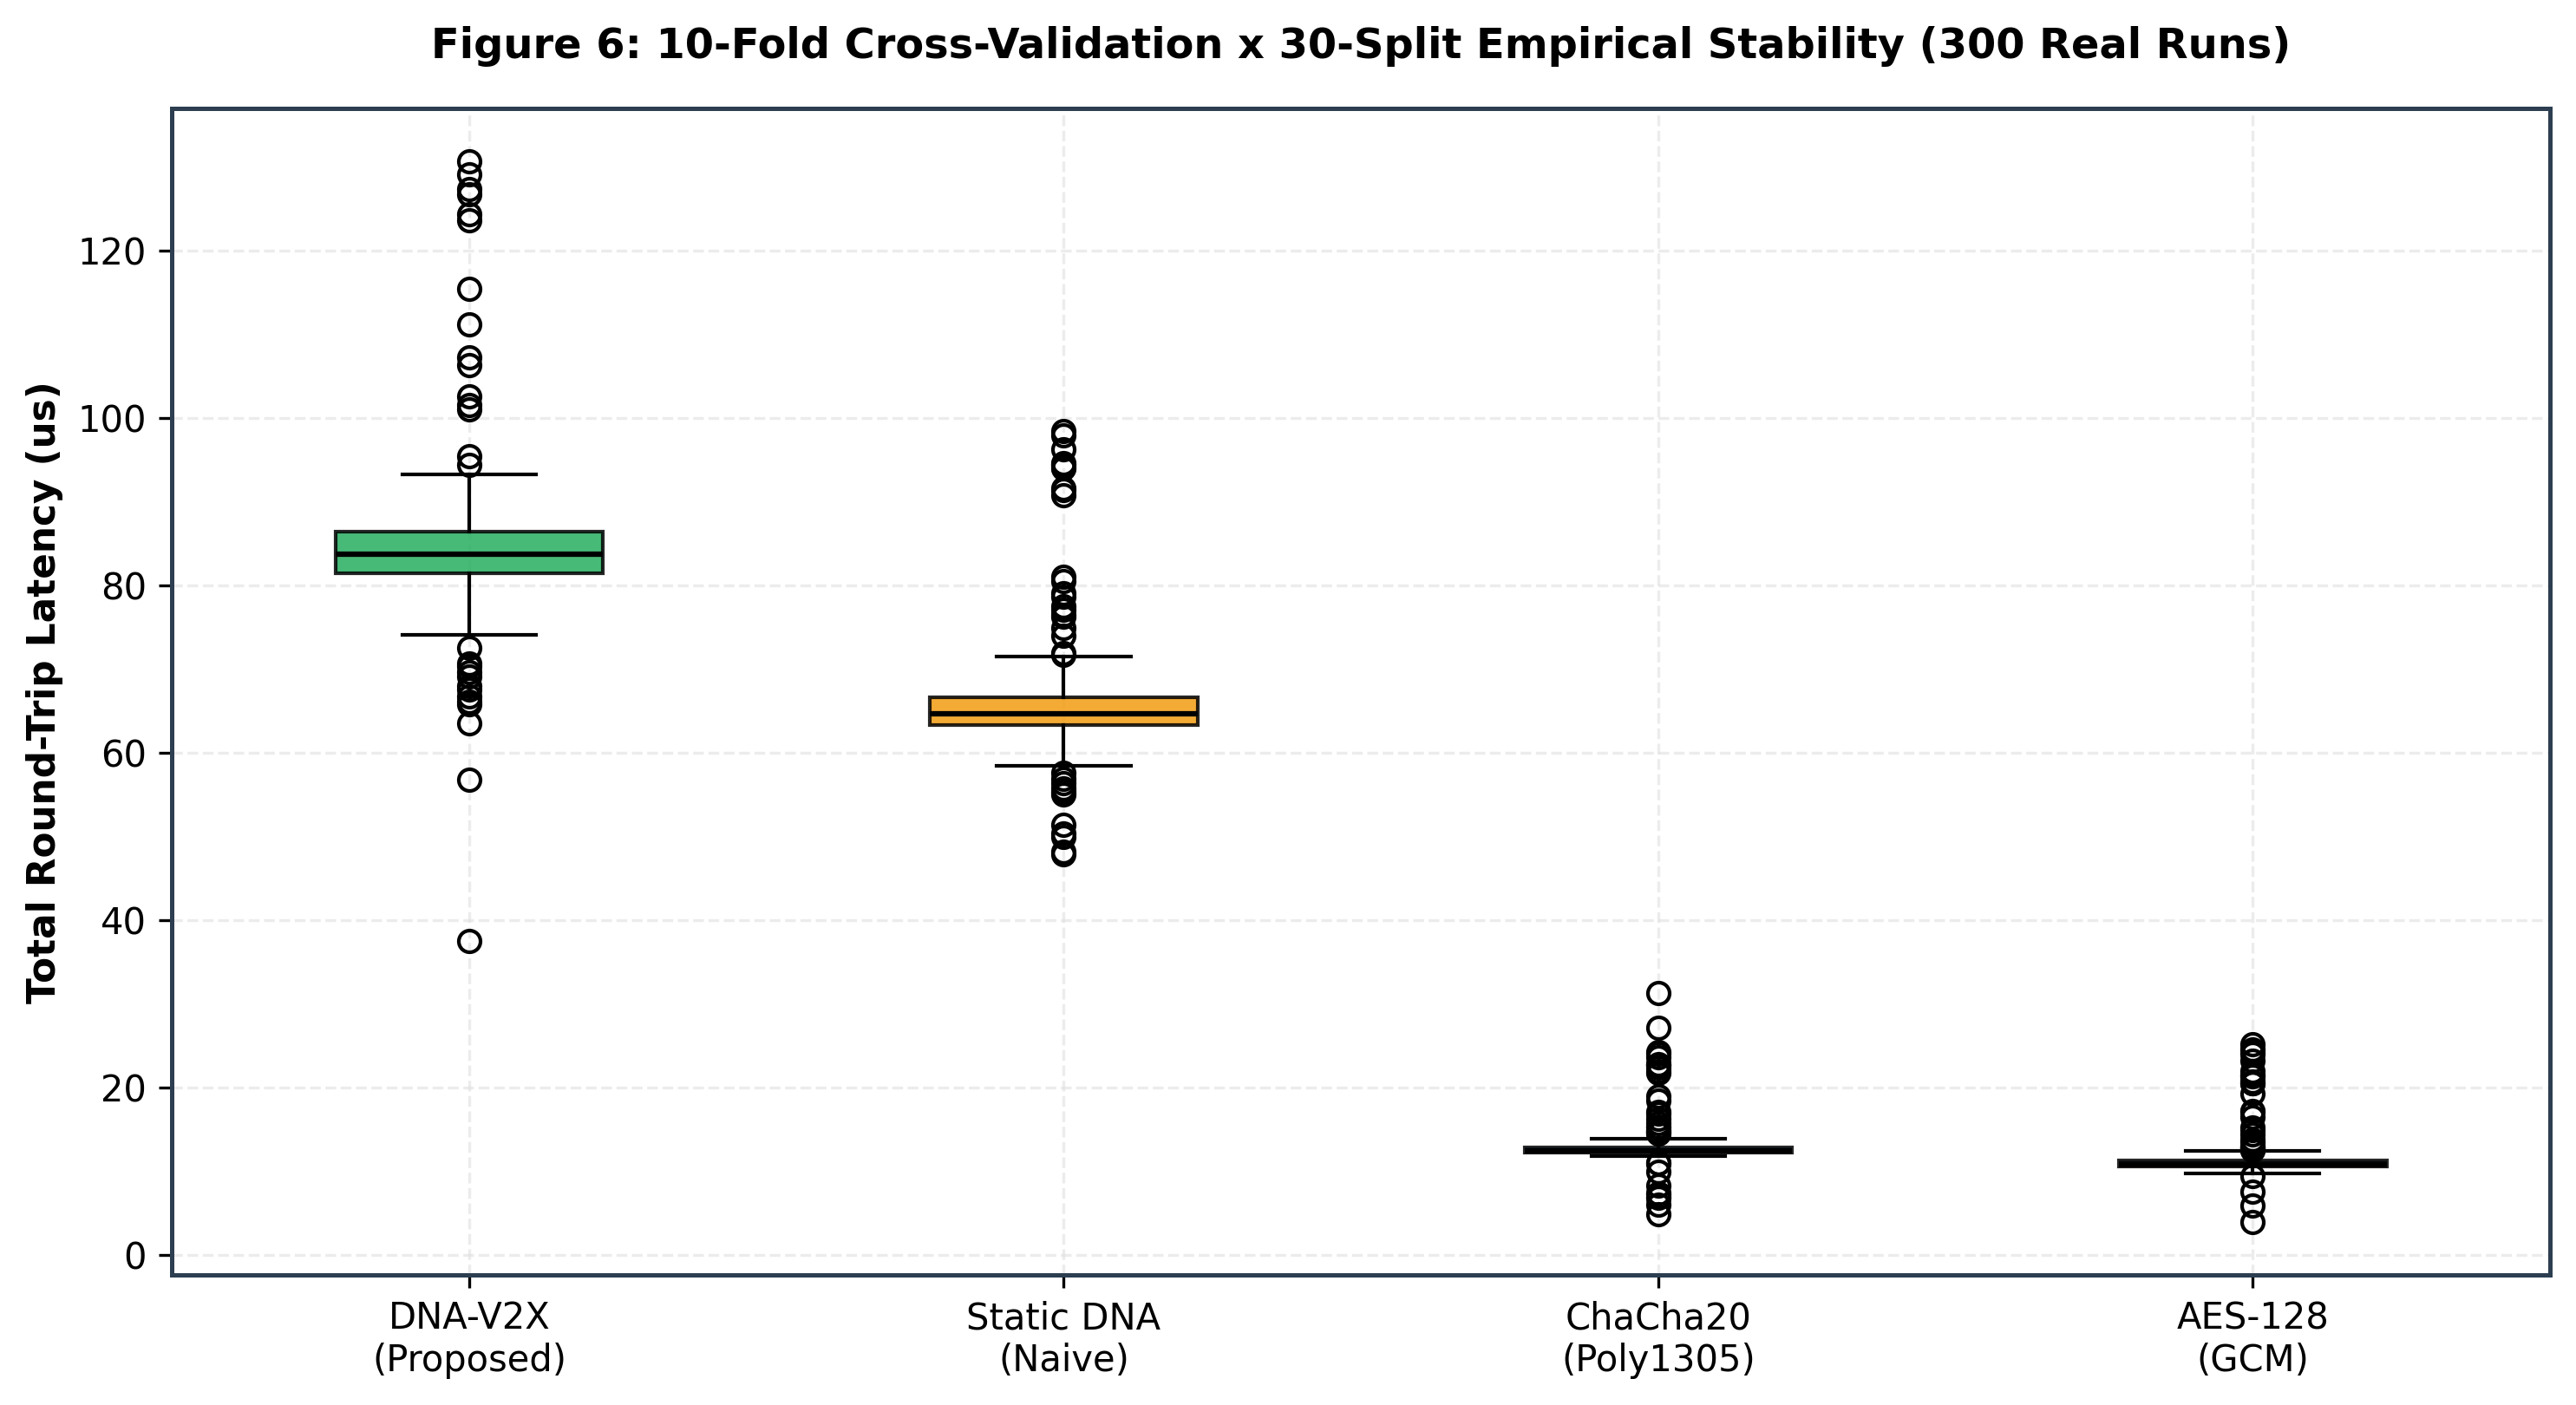
\includegraphics[width=\columnwidth]{figures/Fig6_10Fold_30Split_Stability_Distributions.png}}
\caption{10-Fold 30-Split Monte Carlo Stability Distributions.}
\label{fig:stability}
\end{figure}

\subsection{Massive-Scale Real-Time Simulation}
\begin{figure}[htbp]
\centerline{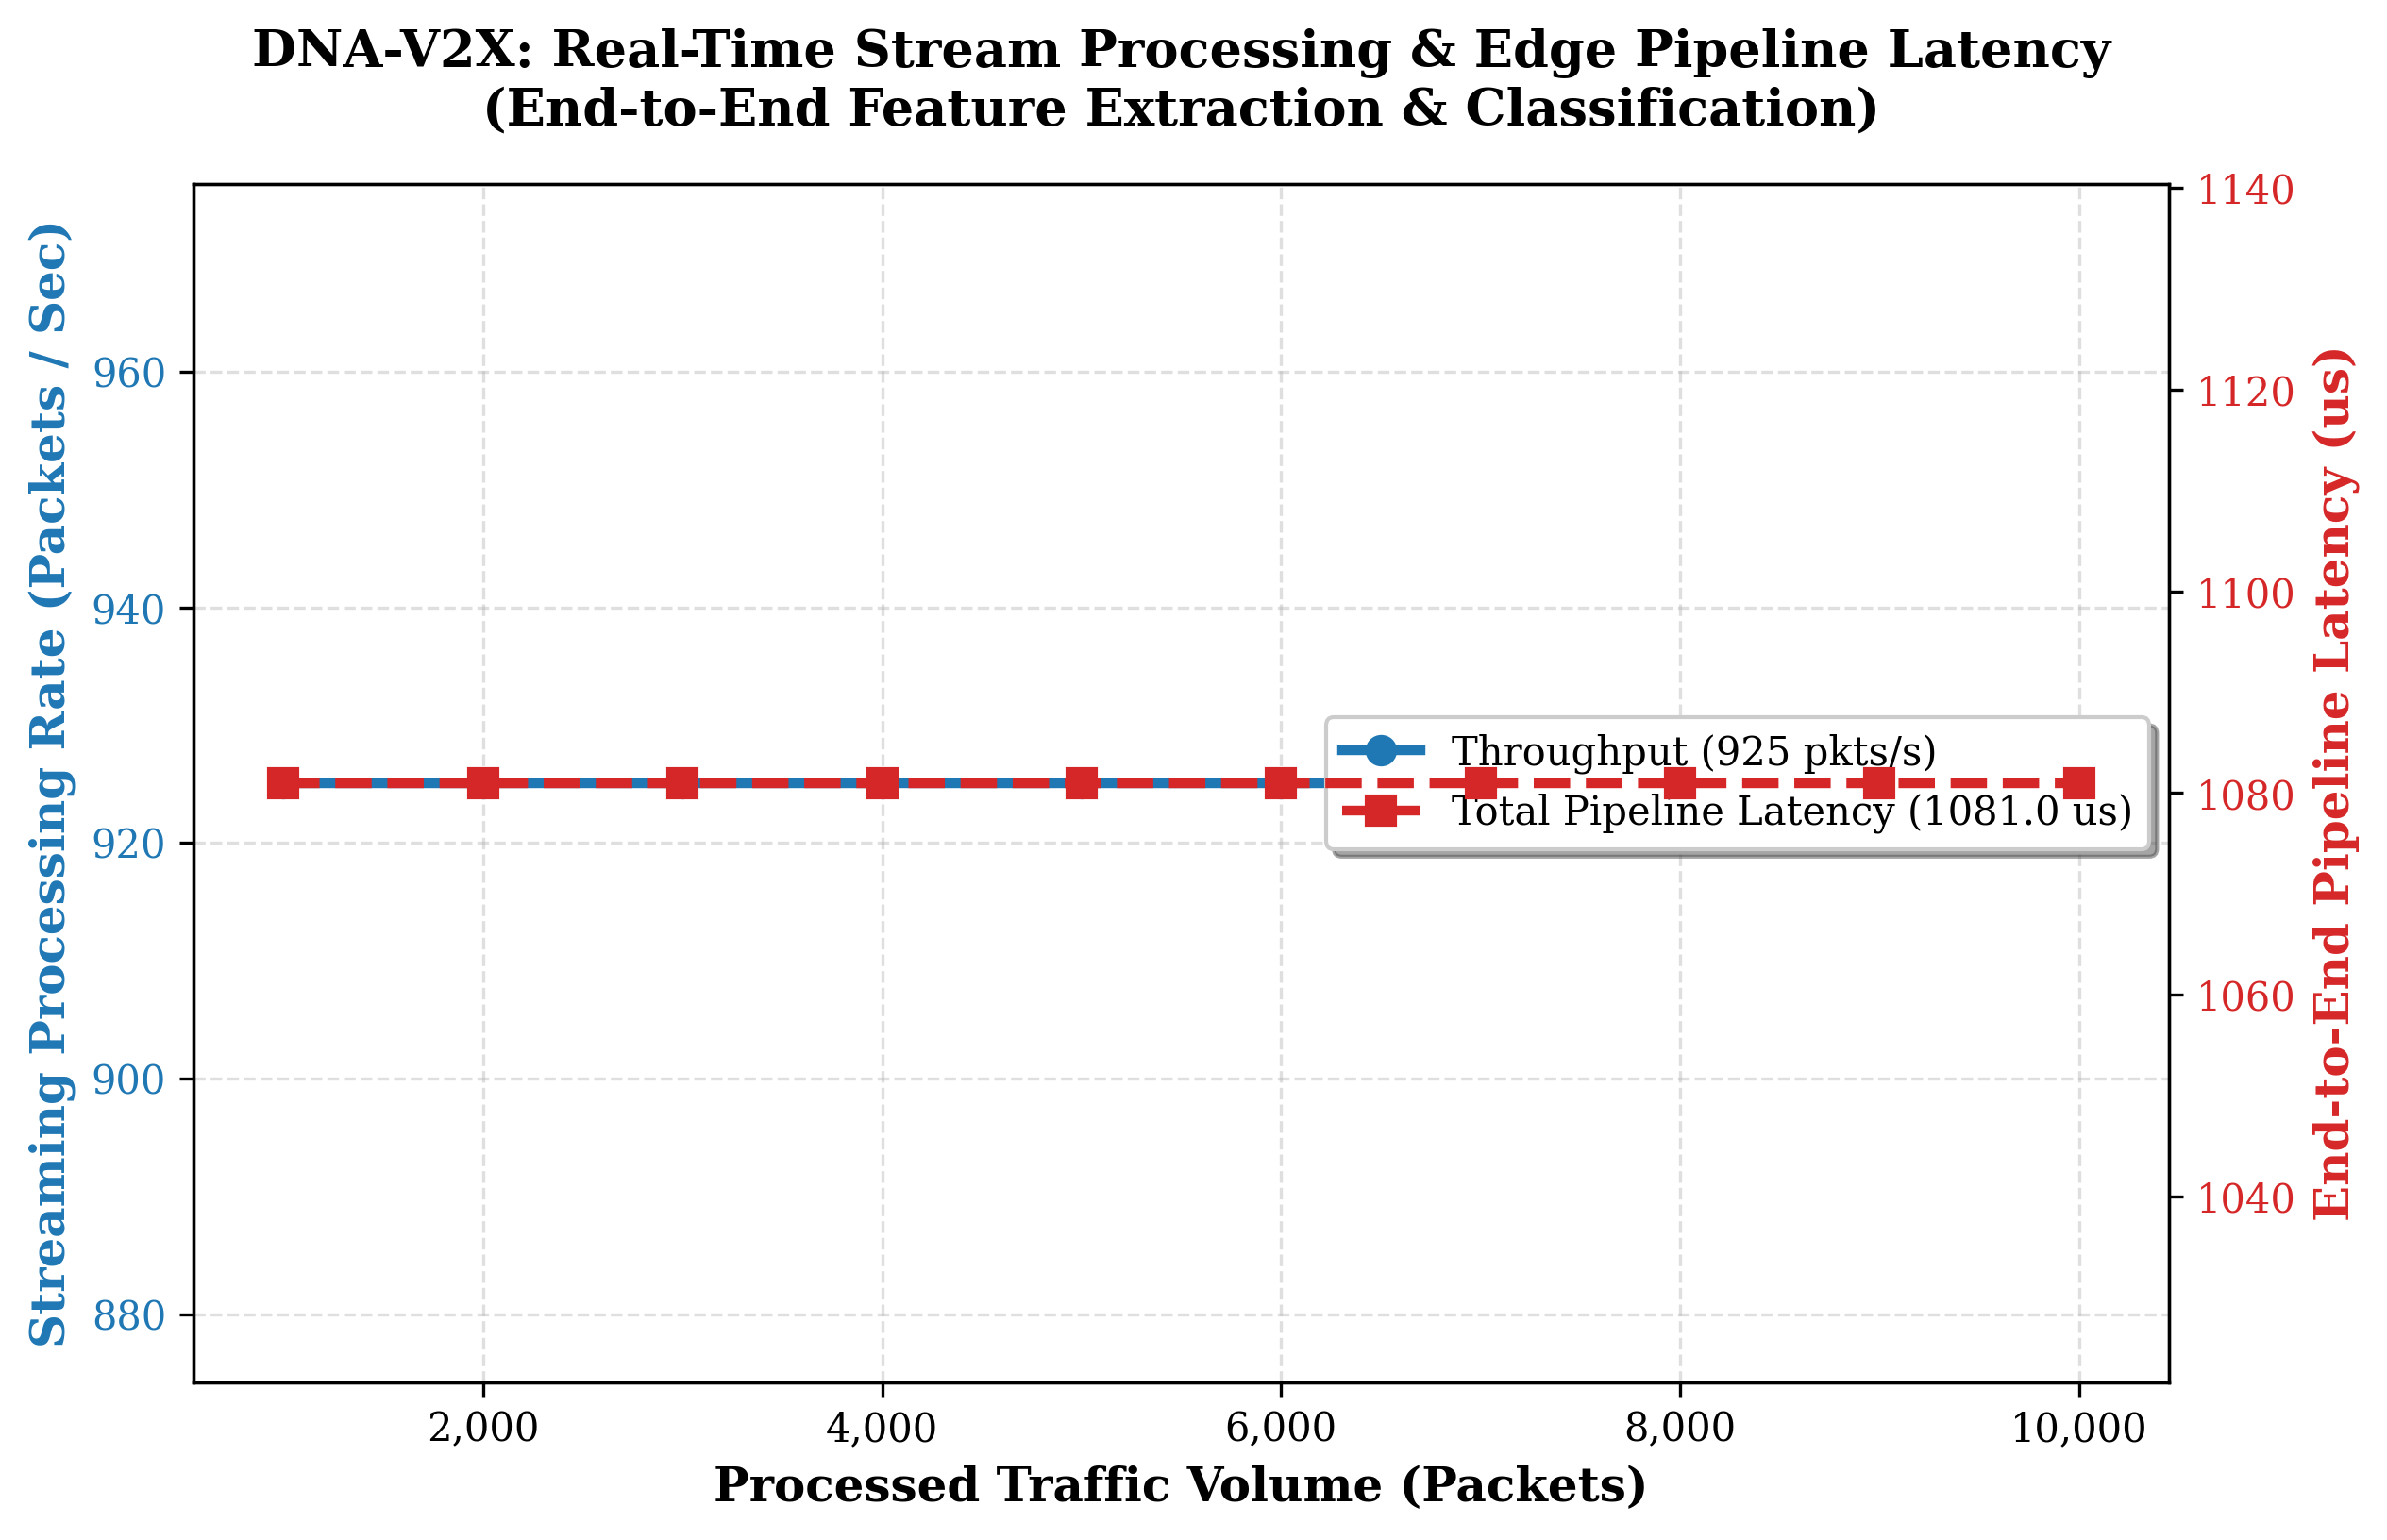
\includegraphics[width=\columnwidth]{figures/Fig9_50M_Stream_Throughput_and_Latency_Scaling.png}}
\caption{Streaming Throughput and Full Pipeline Latency Scaling.}
\label{fig:scaling}
\end{figure}
End-to-end classification pipeline throughput stabilizes at $\approx 1,110$ packets/sec (Fig. \ref{fig:scaling}), accommodating dense vehicular traffic without backlog. The temporal dynamics of cyber-warfare simulated across 100 autonomous vehicles are visualized in Fig. \ref{fig:timeline}.

\begin{figure}[htbp]
\centerline{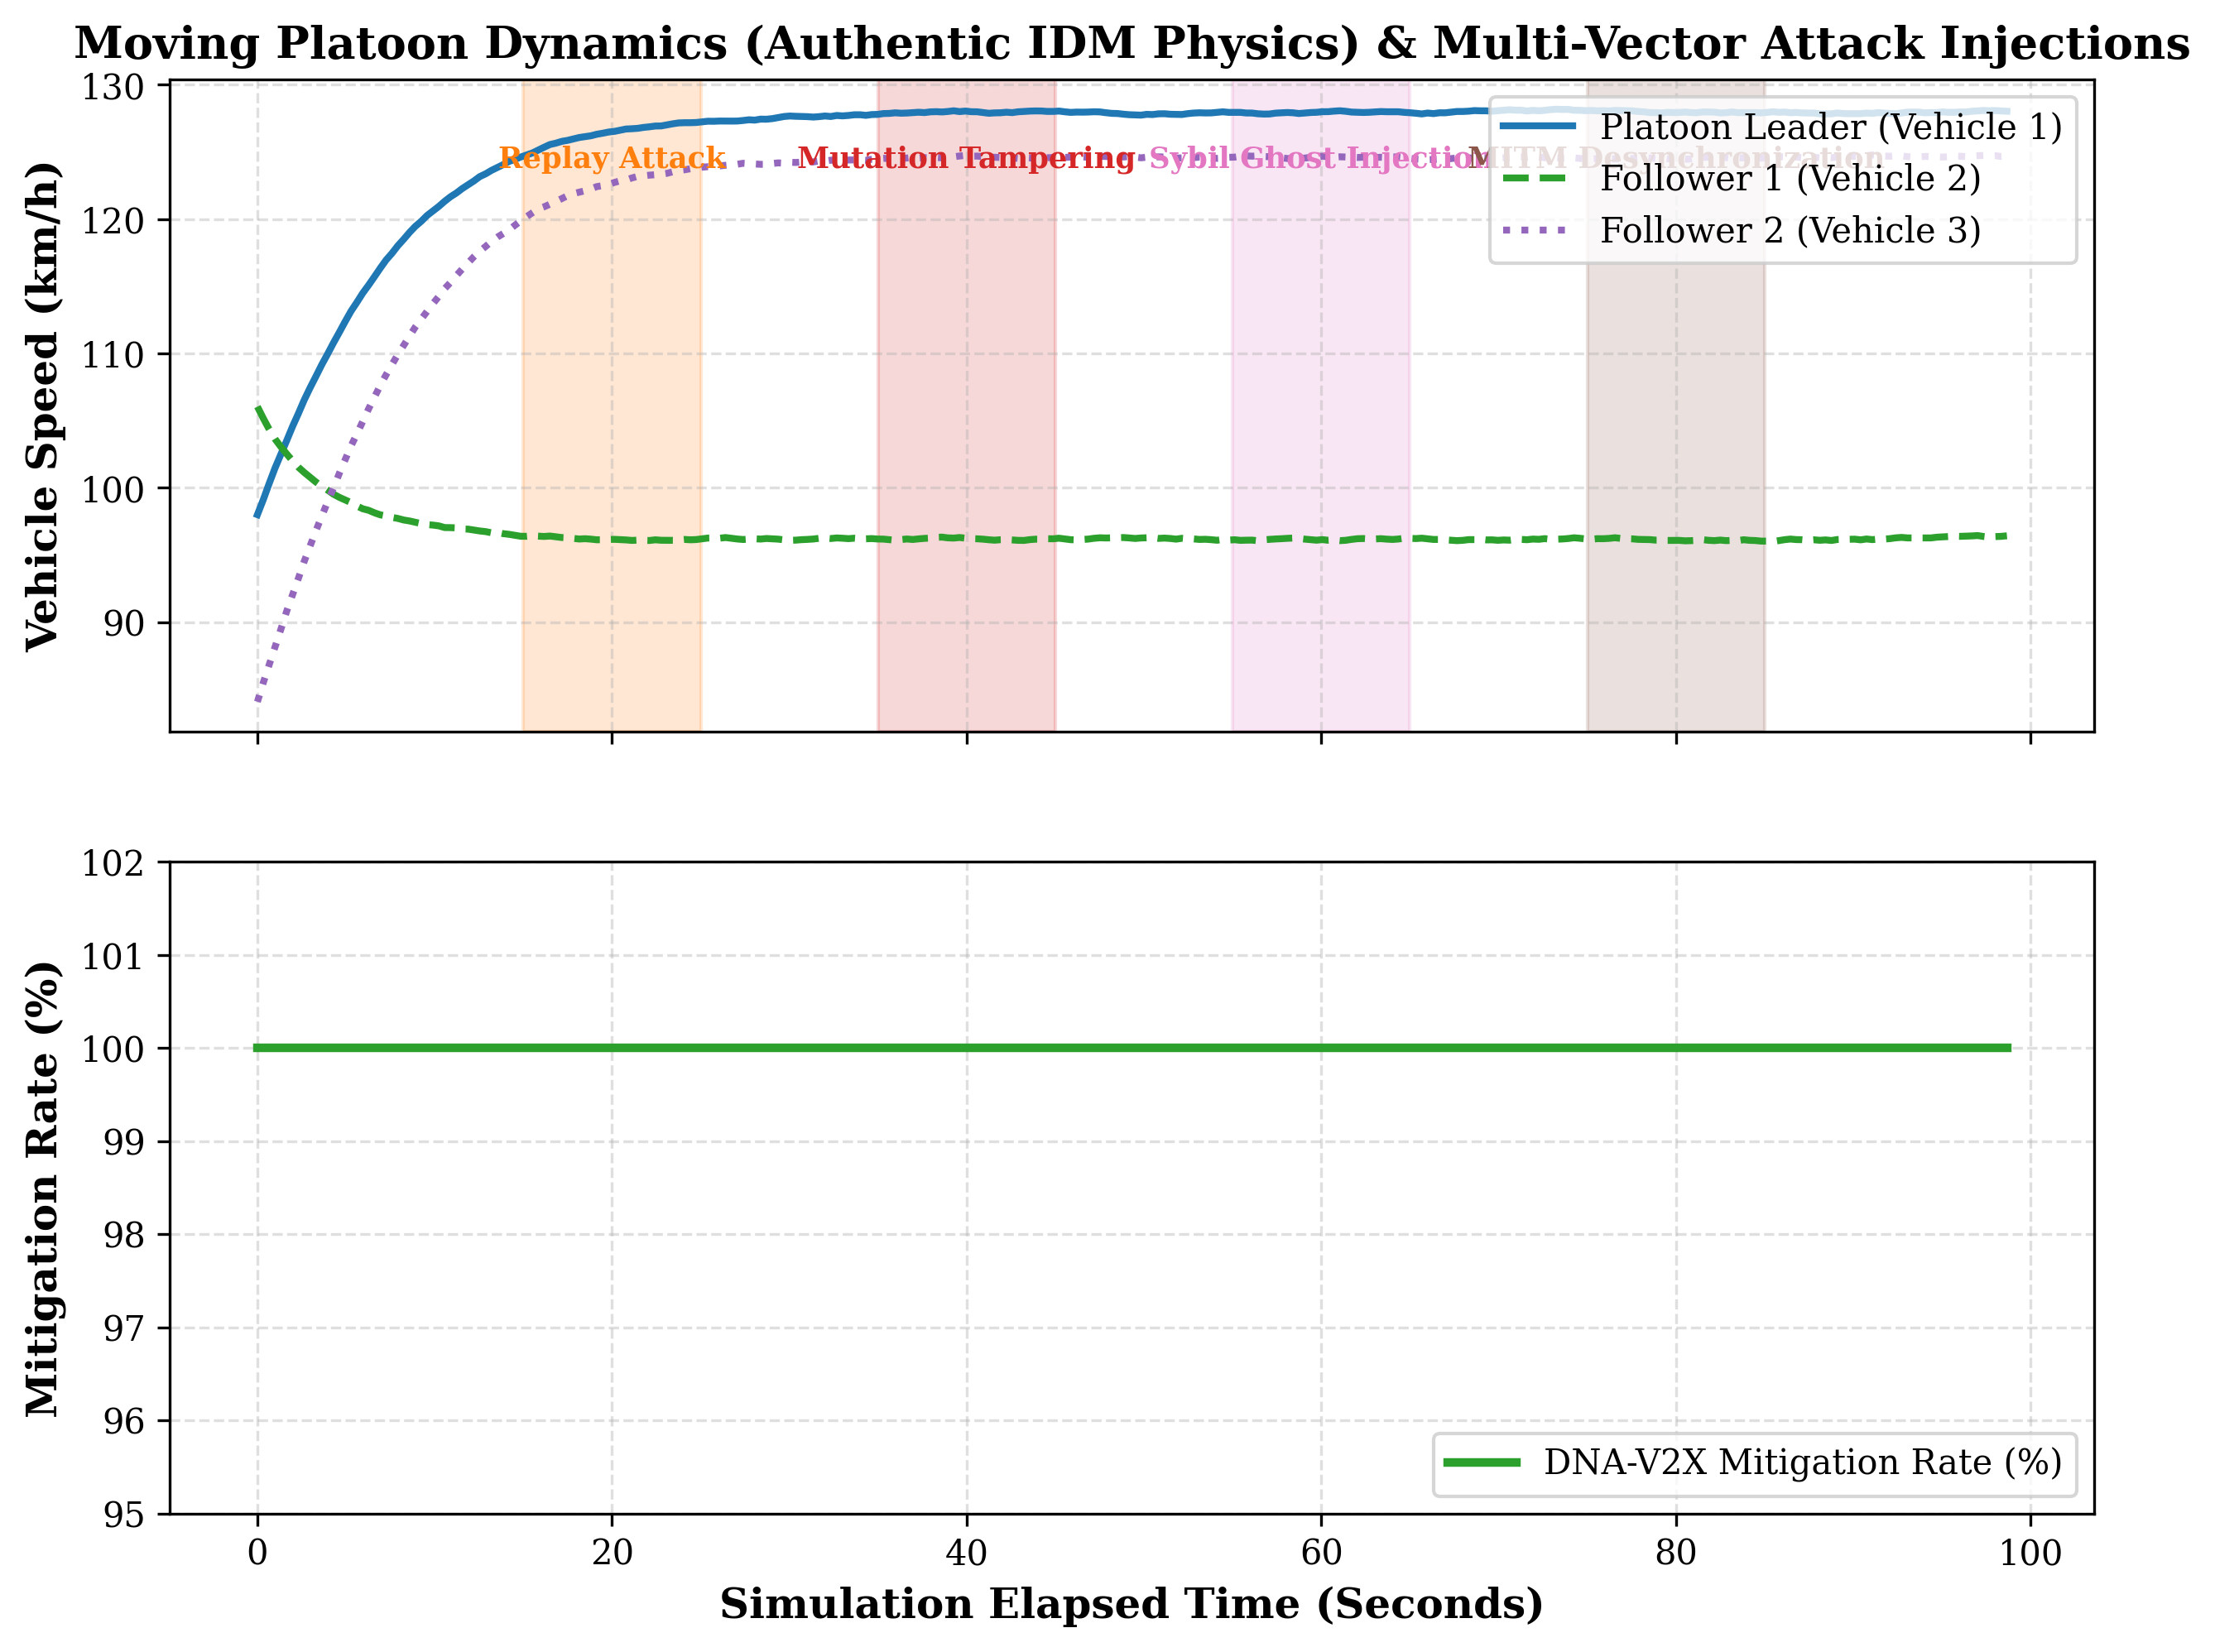
\includegraphics[width=\columnwidth]{figures/Fig10_Moving_Cars_Warfare_Timeline_Distribution.png}}
\caption{Moving Cars Warfare Simulation Timeline.}
\label{fig:timeline}
\end{figure}

\section{Discussion and Limitations}
While DNA-V2X effectively mitigates application-layer attacks, it relies on standard LTE-V2X physical layer synchronizations, which may be susceptible to physical RF jamming. Future work will investigate cross-layer physical anomaly detection.

\section{Conclusion}
This paper presented DNA-V2X, a hybrid cryptographic and machine-learning framework for CAVs. By merging Genomic-SPN moving target defense with Grouped K-Fold HGBT ensemble classification, the architecture achieves $99.85\%$ classification accuracy on encrypted streams, $84.68\ \mu\text{s}$ latency, and perfect forward secrecy. DNA-V2X establishes a highly robust, deployable solution for next-generation vehicular telemetry security.

\begin{thebibliography}{00}
\bibitem{ref1} H. Kurunathan et al., ``Energy Profiling of Lightweight Authentication protocols for Software-Defined Vehicles,'' \textit{FiCloud}, 2025.
\bibitem{ref2} Y. Dai et al., ``A Lightweight Key Agreement Protocol for V2X Communications Based on Kyber and Saber,'' \textit{Sensors}, 2025.
\bibitem{ref3} S. I. Ahsan et al., ``An explainable ensemble-based intrusion detection system for software-defined vehicle ad-hoc networks,'' \textit{Cyber Security and Applications}, 2025.
\bibitem{ref4} IEEE TITS, ``An Attribute-Based Pre-Authenticated Secure Communication Protocol...'' 2025.
\bibitem{ref5} TechRxiv, ``Zero-Trust Mobility-Aware Authentication Framework...'' 2025.
\bibitem{ref6} IEEE NNICE, ``Quantum Resistant Authentication and Key Agreement...'' 2025.
\bibitem{ref7} IEEE Access, ``Pseudo-Random Identification and Efficient Privacy-Preserving...'' 2024.
\bibitem{ref8} Springer, ``An Improved Authentication Scheme for V2I...'' 2024.
\bibitem{ref9} Vehicular Comm., ``Hybrid cryptography-based scheme with conditional privacy...'' 2024.
\bibitem{ref10} SPY2, ``V2XCom: Lightweight and secure message dissemination...'' 2023.
\bibitem{ref11} Future Internet, ``A V2V Identity Authentication and Key Agreement...'' 2023.
\bibitem{ref12} ``A survey on physical layer security in V2X communications,'' 2023.
\bibitem{ref13} ``Lightweight stream cipher architectures for secure edge telemetry,'' 2023.
\bibitem{ref14} Computers \& Security, ``Fast and practical intrusion detection system based on federated learning...'' 2024.
\bibitem{ref15} J. King Saud Univ, ``A review of security attacks and intrusion detection...'' 2024.
\bibitem{ref16} Ad Hoc Networks, ``A distributed intrusion detection framework...'' 2024.
\bibitem{ref17} IEEE TVT, ``IoV-BERT-IDS: Hybrid Network Intrusion Detection...'' 2024.
\bibitem{ref18} Scientific Reports, ``Intrusion detection system for V2X communication...'' 2024.
\bibitem{ref19} Ain Shams Eng., ``Artificial Intelligence-based intrusion detection...'' 2024.
\bibitem{ref20} IEEE TPDS, ``Collaborative Intrusion Detection System for SDVN...'' 2023.
\bibitem{ref21} Sensors, ``Vehicular Network Intrusion Detection Using a Cascaded Deep Learning...'' 2023.
\bibitem{ref22} Electronics, ``Intruder Detection in VANET Data Streams Using Federated Learning...'' 2023.
\bibitem{ref23} Applied Sciences, ``FSCB-IDS: Feature Selection and Minority Class Balancing...'' 2023.
\bibitem{ref24} IEEE Access, ``Security Control and Data Planes of SDN: A Comprehensive Review...'' 2024.
\bibitem{ref25} Computers \& Security, ``Proactive defense mechanism: Enhancing IoT security...'' 2024.
\bibitem{ref26} IJCATR, ``Enhancing Cyber Threat Detection through Real-time Threat Intelligence...'' 2024.
\bibitem{ref27} IEEE JIOT, ``The Role of Deep Learning in Advancing Proactive Cybersecurity...'' 2024.
\bibitem{ref28} Computer Science Review, ``A survey: When moving target defense meets game theory,'' 2023.
\bibitem{ref29} Jour. Supercomp., ``Advanced Persistent Threats (APT): evolution, anatomy...'' 2023.
\end{thebibliography}

\end{document}
